\documentclass[14pt, a4paper]{extreport}

\usepackage[utf8]{inputenc}
\usepackage{times}
\usepackage[T5]{fontenc}
\usepackage[vietnamese=nohyphenation]{hyphsubst}
\usepackage[vietnamese]{babel}
\usepackage[bottom=2cm, top=2cm, left=3cm, right=2cm]{geometry}
\usepackage{graphicx}
%draw
\usepackage{tikz}
\usetikzlibrary{calc}
\usepackage{enumitem}
\usepackage{eso-pic}
\usepackage{indentfirst}
%change \chapter and \section style
\usepackage[explicit]{titlesec}
\usepackage{romannum}
%show source code
\usepackage{listings}
%rotate images
\usepackage{rotating}
%tabular with wrap
\usepackage{tabularx}
\usepackage{fancyhdr}
%multi dot
\usepackage{multido}
\titleformat{\chapter}
    {\bfseries\centering}
    {CHƯƠNG \Romannum{\thechapter}. \MakeUppercase{#1}}
    {0.3em}{}
\titleformat{\section}{\bfseries}{\thesection. #1}{0.3em}{}
\titleformat{\subsection}{\bfseries}{\thesubsection. #1}{0.3em}{}
\titleformat{\subsubsection}{\bfseries}{\thesubsubsection. #1}{0.3em}{}

\titlespacing{\chapter}{0pt}{\parskip}{-\parskip}
\titlespacing{\section}{0pt}{\parskip}{-\parskip}
\titlespacing{\subsection}{0pt}{\parskip}{-\parskip}
\titlespacing{\subsubsection}{0pt}{\parskip}{-\parskip}
\renewcommand{\headrulewidth}{0pt}

\newcommand{\clearHeading}{
    \clearpage
    \fancyhead[]{}
    \cfoot[]{\thepage}
    \setcounter{page}{1}
}
\makeatletter
\renewcommand{\maketitle}{
    \begin{titlepage}
        \newgeometry{top=2cm,bottom=2cm,left=2cm,right=2cm}
        \AddToShipoutPicture*{
            \AtTextCenter{
                \makebox(0,0)[c]{
                    \begin{tikzpicture}
                        \draw[line width=1pt](0,0)
                            rectangle(\textwidth+2*0.3cm,\textheight+2*0.3cm);
                    \end{tikzpicture}
                }
            }
        }
        \begin{center}
            
            {\fontsize{13}{15.6}\selectfont
                ĐẠI HỌC CÔNG NGHỆ THÔNG TIN VÀ TRUYỀN THÔNG THÁI NGUYÊN\\
                \textbf{KHOA: CÔNG NGHỆ THÔNG TIN}\\
                \rule{3cm}{1.pt}
            }
            
            \begin{figure}[h!]
                \centering
                
\includegraphics[width=100px]{fig/Logo_ICTU.png}
            \end{figure}
            
            {\fontsize{18}{21.6}\selectfont\textbf{BÁO CÁO\\
                THỰC TẬP CHUYÊN NGÀNH}}
            
            \vfill %%%%%%%%%%%%%%%%%%%%%%%%%%%%%%%%%%%%%%%%%%%%%%%%%%%%%%%%%%%%
            
            \textbf{ĐỀ TÀI\\}
            {\fontsize{18}{21.6}\selectfont\textbf{\MakeUppercase\@title}}
            
            \vfill %%%%%%%%%%%%%%%%%%%%%%%%%%%%%%%%%%%%%%%%%%%%%%%%%%%%%%%%%%%%
            \begin{tabular} {l l}
                Sinh viên thực hiện: & \MakeUppercase\@author \\
                Lớp: & CNTT-K14C \\
                Giáo viên hướng dẫn: & ThS. NGÔ THỊ LAN
            \end{tabular}
            \vfill

            {\fontsize{14}\selectfont\textbf{Thái Nguyên, 05 tháng 04 năm 2019}}
        \end {center}
    \end{titlepage}
}
\makeatother


\renewcommand{\baselinestretch}{1.5}
\setlength{\headheight}{17pt}
\lstset{basicstyle=\ttfamily,breaklines=true}

\title{xây dựng website bán linh kiện điện tử cho cửa hàng Nam Hải}
\author{Nguyễn Đăng Hải}
\begin{document}
\maketitle
\pagenumbering{arabic}
\pagestyle{fancyplain}
\cfoot[]{}
\tableofcontents

\clearHeading
\pagestyle{fancyplain}
\cfoot[]{}
    \addcontentsline{toc}{chapter}{Lời mở đầu}
    \begin{center}
        \textbf{Lời mở đầu}
    \end{center}
    Trước sự cạnh tranh ngày một khốc liệt của thị trường, việc chỉ mở cửa hàng mà buôn bán thông thường không còn phù hợp nữa, thay vào đó các cửa hàng, doanh nghiệp ngày nay thường khá quan trọng đến sự hiện diện của mình trên mạng, việc tăng sự hiện diện của mình trên mạng không chỉ giúp cửa hàng, doanh nghiệp nhanh chóng mở rộng sự hiện diện của mình một cách nhanh chóng mà còn giúp cửa hàng, doanh nghiệp tiếp cận được nhiều đối tượng tiềm năng hơn. Với lượng người sử dụng internet tại Việt Nam vào năm 2018 là 64 triệu người (tương đương với 67\% dân số) theo cdnvietnam.com Việc đầu tư vào sự hiện diện của mình trên mạng là rất cần thiết.
    
    Cửa hàng Nam Hải là một cửa hàng buôn bán linh kiện điện tử có địa chỉ tại Lào Cai, hiện tại họ đang mong muốn tăng cường sự hiện diện của mình trên mạng bằng cách triển khai một website bán hàng với những chức năng giúp họ có thể đăng sản phẩm, quản lý đơn hàng, thêm các chương trình khuyến mãi, ngoài ra website cũng phải có giao diện đẹp mắt, hoạt động ổn định.
    
    Từ những nhu cầu trên, em chọn đề tài “abcxyz” đề thực tập chuyên ngành với mục tiêu xây dựng một website đáp ứng được những yêu cầu của cửa hàng cũng như áp dụng những kiến thức đã được học vào thực tế.
    
    Em xin trân thành cảm ơn.

\cfoot{\thepage}
\chapter{Cơ sở lý thuyết}
\section{HTML}
\subsection{Giới thiệu ngôn ngữ:}
HTML là ngôn ngữ được dùng để định nghĩa cấu trúc của một trang web, được ra đời vào năm 1990, cho tới hiện tại HTML đã trả qua năm phiên bản, tại phiên bản hiện tại (HTML5) HTML được bổ sung thêm nhiều tính năng mới như WebRTC, trình chơi video, drag \& drop, service worker,... giúp xây dựng các ứng dụng web đa dạng và mạnh mẽ hơn trước, ngoài ra HTML còn cung cấp một số thẻ semantic giúp bọ của những công cụ tìm kiếm như Google, Yandex,... đễ dàng đọc cấu trúc và các thành phần quan trọng của website hơn. Điều này mang tới lợi ích cho việc SEO nhưng không bắt buộc lập trình viên phải sử dụng.\par
\subsection{Cú pháp cơ bản}
Cú pháp và thẻ trong HTML không cần độ chính xác tuyệt đối để chạy được
giống như những ngôn ngữ như XML, XHTML thay vào đó những thẻ hay cú pháp khác thường mà trình duyệt không hỗ trợ thì sẽ bị trình duyệt lờ đi và không có tác dụng gì, việc này giúp các trình duyệt phiên bản cũ vẫn có thể xem được nhưng trang HTML phiên bản cao hơn tuy rằng những trình duyệt này sẽ không thể sử dụng được các tính năng mới được cung cấp (Đảm bảo tính tương thích ngược).\par
Hiện nay HTML đang muốn hướng lập trình viên tạo ra những trang web mới sử dụng các thẻ semantic (ngữ nghĩa) thay cho việc dùng <div> hay <span>vì hai thẻ này không diễn tả được nhiều về các thành phần của một trang web, một số thẻ ngữ nghĩa thường dùng là:
\begin{center}
\begin{tabular}{|l|l|}
    \cline{1-2}
    \textbf{Thẻ} & \textbf{Chức năng} \\ \cline{1-2}
    <article> & Liệt kê các bài viết \\ \cline{1-2}
    <aside> & Phần nội dung bên lề \\ \cline{1-2}
    <figure> & Chứa các hình ảnh, biểu đồ, .... \\ \cline{1-2}
    <figcaption> & Chứa phần mô tả hình ảnh cho thẻ <figure> \\ \cline{1-2}
    <header> & Phần đầu trang web \\ \cline{1-2}
    <footer> & Phần chân trang \\ \cline{1-2}
    <main> & Phần nội dung chính của tài liệu \\ \cline{1-2}
    <mark> & Phần văn bản được đánh dấu, làm nổi bật \\ \cline{1-2}
    <nav> & Phần thanh định hướng \\ \cline{1-2}
    <section> & Định nghĩa các phân đoạn trong trang web \\ \cline{1-2}
    <details> & Chứa nội dung chi tiết, người dùng có thể xem hay ẩn đi \\ \cline{1-2}
    <summary> & Nêu tóm lược nội dung, kết hợp với thẻ <details> \\ \cline{1-2}
    <time> & Thời gian, có thể là thời gian đăng bài, thời gian chỉnh sửa, ... \\ \cline{1-2}
    <video> & Nhúng nội dung video vào trang web \\ \cline{1-2}
\end{tabular}
\end{center}

Một file HTML thường có phần mở rộng là \textbf{*.html} và có cấu trúc như sau:
\lstset{language=Html}
\begin{center}
\begin{lstlisting}[frame=single]
 <html>
 <head>
    <title>Html example</title>
    <meta charset="utf-8">
 </head>
 <body>
    Hello world
 </body>
 </html>
\end{lstlisting}
\end{center}
Cặp thẻ <html><html> được dùng để bao toàn bộ nội dung file html, cặp thẻ <head></head> dùng để chứa khai báo về trang web như tiêu đề, nối các file css, các siêu nội dung (meta-content),... Cuối cùng là cặp thẻ <body> dùng để chứa nội dung của toàn bộ trang web.
\section{CSS}
CSS là ngôn ngữ dùng để bổ sung các thuộc tính hiển thị cho trang web về mặt màu sắc và cách thức hiện thị của nội dung trên trang web bằng cách định nghĩa các thuộc tính cho những thẻ HTML trong trang web, các thuộc tính này phải được trình duyệt hỗ trợ, trong trường hợp cố tình dùng những thuộc tính không được hỗ trợ, trình duyệt sẽ lờ những thuộc tính đó và chỉthực thi các thuộc tính được hỗ trợ.\par
Hiện tại phiên bản mới nhất của CSS là CSS 3 với rất nhiều thuộc tính mới giúp việc căn chỉnh các thành phần của trang web dễ dàng hơn, một số tính năng đáng nói có thể kể đến như:

\begin{table}[h!]
\centering
\begin{tabular}{|l|l|}
    \cline{1-2}
    \textbf{Thuộc tính} & \textbf{Chức năng}\\ \cline{1-2} 
    flexbox & Căn chỉnh vị trí phần tử theo một chiều cố định (ngang hoặc dọc)\\ \cline{1-2}
    Gird layout & Căn chỉnh vị trí của phần tử theo cả chiều ngang lẫn chiều dọc\\ \cline{1-2}
\end{tabular}
\end{table}

Hiện tại cả hai thuộc tính này đều đã được tích hợp trong Bootstrap 4 một framework css rất nổi tiếng và được nhiều lập trình viên sử dụng.
\section{Bootstrap}
Bootstrap là một framework css, hiểu một cách đơn giản thì Bootstrap là những class css được định nghĩa sẵn thuộc tính, việc dùng các class được Bootstrap định nghĩa sẵn giúp lập trình viên nhanh chóng tạo được những trang web có giao diện đẹp, hiện đại mà không phải viết nhiều css.\par
Việc dùng các class có sẵn giúp tạo lập tiêu chuẩn chung giữa các lập trình viên về việc đặt tên class vì thường khi sử dụng css thuần để viết, mỗi lập trình viên có thể viết những tên class không thống nhất dẫn tới việc các thuộc tính ghi đè lên nhau và vô hình chung làm kích thước cũng như độ minh bạch của file css ngày một giảm đi và khó để bảo trì hơn.\par
Một vấn đề khác khi viết css thuần là lập trình viên kinh nghiệm khi phải xử lý fallback cho những trình duyệt khác nhau và những phiên bản trình duyệt cũ cũng như xử lý media query cho phù hợp với nhiều cỡ màn hình khác nhau.\par
Việc cài đặt Bootstrap cũng tương đối đơn giản, chỉ cần thêm những dòng sau vào giữa cặp thẻ <head></head> trong file html

\lstset{language=Html}
\vspace{-1em}
\begin{lstlisting}[frame=single]
 <link rel="stylesheet" href="http://maxcdn.bootstrapcdn.com/bootstrap/3.3.4/css/bootstrap.min.css">
\end{lstlisting}

Và những dòng sau và trước thẻ đóng </body>

\vspace{-1em}
\begin{lstlisting}[frame=single]
 <script src="https://ajax.googleapis.com/ajax/libs/jquery/1.11.1/jquery.min.js"></script>
 <script src="http://maxcdn.bootstrapcdn.com/bootstrap/3.3.4/js/bootstrap.min.js"></script>
\end{lstlisting}

File html sau khi cài đặt Bootstrap sẽ nhìn như sau

\begin{center}
\vspace{-2em}
\begin{lstlisting}[frame=single]
 <html>
 <head>
    <title>Html example</title>
    <meta charset="utf-8">
    <link rel="stylesheet" href="http://maxcdn.bootstrapcdn.com/bootstrap/3.3.4/css/bootstrap.min.css">
 </head>
 <body>
    Hello world

    <script src="https://ajax.googleapis.com/ajax/libs/jquery/1.11.1/jquery.min.js"></script>
    <script src="http://maxcdn.bootstrapcdn.com/bootstrap/3.3.4/js/bootstrap.min.js"></script>
 </body>
 </html>
\end{lstlisting}
\vspace{-1.5em}
\end{center}

Việc thêm thư viện javascript vào trước đóng thẻ </body> giúp trình duyệt tải và hiển thị html cũng như css trước sau đó mới tải đến Javascript, việc này giúp tránh hiện tượng trang web trắng xóa, không hiển thị nội dung gì khi trình duyệt cố tải những thư viện Javascript.\par
\textbf{Lưu ý:} Phải đặt Jquery trước các thư viện javascript khác vì đa phần những thư viện của Bootstrap đều dùng Jquery và sẽ không hoạt động nếu thiếu Jquery.
\section{PHP}
\subsection{Giới thiệu ngôn ngữ}
Php là một ngôn ngữ chạy ở phía Server (backend) dùng để nhận truy vấn từ người dùng, xử lý và trả về thông tin phù hợp, tuy được coi là một ngôn ngữ có độ bảo mật không được cao xong đây lại là một ngôn ngữ dễ học với cộng đồng hỗ trợ và phát triển đông đảo, hiện tại phần lớn các website trên internet vẫn sử dụng php, Php cũng được sử dụng trong nhiều framework nổi tiếng có thể kể đến như: Joomla, Wordpress, Laravel, Code Igniter,...\par
Tuy là vậy nhưng Php thuần cũng có những nhược điểm như dễ học nhưng không dễ viết, vì php thuần không hề bó buộc lập trình viên phải lập trình theo một tiêu chuẩn nhất định như những ngôn ngữ khác, lập trình viên có thể tùy ý dùng snake\_case để khai báo tên lớp, tên hàm, cũng có thể dùng CamelCase; Tên lớp cũng có thể không giống với tên file dễ gây nhầm lẫn.\par
Từ những vấn đề đó cộng đồng đã cùng đưa ra bộ chuẩn PSR (Php Standards Recommendations) nhằm đưa ra các khuyến nghị để thống nhất cách viết php, tuy nhiên đây cũng chỉ là những khuyến nghị (Recommandations) chứ không được tích hợp vào ngôn ngữ nên những lập trình viên khi lần đầu sử dụng dễ viết ra những chương trình chạy được nhưng lại khó để duy trì và phát triển cũng như khó để hai lập trình viên có thể viết cùng một code base (do phong cách code của mỗi người là khác nhau).
\subsection{Cú pháp cơ bản}
Các file php có phần mở rộng là \textbf{*.php}, tuy nhiểu để trình dịch hiểu được ta cần đặt các đoạn mã Php vào trong cặp thẻ \textbf{<?php} và \textbf{?>} những lệnh được đặt ngoài hai cặp thẻ này đều được coi là văn bản thông thường và được Php trả về dưới dạng file Html.\par
Ngôn ngữ Php được viết dựa vào ngôn ngữ C nên phong cách code mang nhiều hơi hướng C như việc phải dùng dấu \textbf{;} khi kết thúc mỗi dòng code, phân biệt chữ hoa chữ thường, cũng như là một ngôn ngữ hướng chức năng (Tới phiên bản thứ 5 mới hỗ trợ việc lập trình hướng đối tượng)
\lstset{language=Php}
\begin{center}
\vspace{-2em}
\begin{lstlisting}[frame=single]
<?php
    function helloWord()
    {
        echo 'Hello World';
    }
    helloWorld(); //return Hello World
\end{lstlisting}
\end{center}
\section{MySQL}
\subsection{Giới thiệu ngôn ngữ}
MySQL là một hệ cơ sở dữ liệu quan hệ, trong hệ cơ sở dữ liệu quan hệ dữ liệu được biểu dưới dạng các bảng có liên kết với nhau dựa vào khóa chính hay các khóa phụ. Hiện nay có rất nhiều hệ cơ sở dữ liệu quan hệ như: Oracle, Portgre, mariadb (một bản folk của MySQL),... Tuy nhiên lý do MySQL được chọn là vì:
\begin{enumerate}
\vspace{-1em}
\itemsep0em
\item Quy mô cửa hàng không quá lớn, lượng truy vấn dữ liệu không nhiều
\item Được tích hợp sẵn trong Xampp cũng như phần lớn các shared host hiện nay
\item Miễn phí sử dụng
\end{enumerate}
\subsection{Cú pháp cơ bản}
\begin{center}

\begin{tabularx}{\linewidth}{|l|X|}
 \cline{1-2}
 \textbf{Công việc cần làm} & \textbf{câu lệnh} \\ \cline{1-2}
 Lấy thông tin từ bảng & SELECT * FROM tên\_bảng WHERE điều\_kiện \\ \cline{1-2}
 Nhập thông tin vào bảng & INSERT INTO Tên\_bảng (tên\_cột\_1, tên\_cột\_2, tên\_cột\_3,...) VALUES (giá\_trị\_cột\_1, giá\_trị\_cột\_2, giá\_trị\_cột\_3,...)\\ \cline{1-2}
 Xóa thông tin khỏi bảng & DELETE FROM Tên\_bảng WHERE Điều\_kiện\\ \cline{1-2}
 Cập nhật thông tin bảng & UPDATE Tên\_bảng SET cột\_1 = giá\_trị\_mới, cột\_2 = giá\_trị\_mới, cột\_n = giá\_trị\_mới WHERE điều\_kiện\\ \cline{1-2}
\end{tabularx}
\end{center}

\chapter{Phân tích thiết kế hệ thống}
\section{Khảo sát hiện trạng của hệ thống}
\subsection{Sơ lược về cửa hàng}
Tên cửa hàng: Linh kiện điện tử Nam Hải\par
Trụ sở: 030, đường Hoàng liên, đoạn gần ngân hàng Viettinbank, phường Kim Tân, Thành phố Lào Cai.\par
Cửa hàng Nam Hải được thành lập vào năm 2017 với một cơ sở duy nhất với hai nhân viên kiêm chủ cửa hàng.\par
Cửa hàng chuyên kinh doanh về các loại linh kiện điện tử, vi mạch điều khiển, sạch pin, ... Đối tượng mà cửa hàng nhắm tới là những người có đam mê về công nghệ, robot, tự động hóa, sinh viên các trường công nghệ.\par
Hiện tại do quy mô vẫn còn nhỏ nên việc quản lý cửa hàng chỉ là thông qua giấy tờ, hóa đơn, sổ sách.
\subsection{Thực trạng cửa hàng}
\begin{itemize}
    \item\textbf{Khâu nhập hàng:}\par
    \vspace{-1em}
    \begin{itemize}
        \item Việc nhập hàng thường là nhập trực tiếp từ các lái buôn bên trung quốc, thường mua sỉ mỗi sản phẩm một lượng nhất định phụ thuộc vào sản phẩm nào bán chạy nhất trong những tháng trước đó.
        \item Các sản phẩm thường nhập
            \begin{itemize}
                \item Các sản phẩm được tiêu thụ mạnh trong tháng, quý
                \item Các sản phẩm đang nổi theo trend
            \end{itemize}
        \item Các yếu tố khi cửa hàng nhập sản phẩm
            \begin{itemize}
                \item Ngày nhập
                \item Số lượng sản phẩm nhập vào
                \item Nhà phân phối (nếu có)
                \item Các thông số đi kèm (kích thước, chức năng nổi bật, ...)
                \item Gía thành mỗi sản phẩm
            \end{itemize}
        \item Các thông số nêu trên đều được cửa hàng lưu lại vào sổ nhập hàng để tiện theo dõi
    \end{itemize}
    \item\textbf{Khâu bán hàng:}\par
        \begin{itemize}
        \item Việc bán hàng được thực hiện một cách trực tiếp, khách hàng sẽ tìm đến tận cửa hàng để chọn mua sản phẩm.
        \item Thống kê doanh số bán hàng không có được con số chính xác vì khách hàng đến mua không thường xuyên và cũng chỉ mua nhỏ lẻ một vài sản phẩm.
        \item Thông tin về khách hàng không được lưu lại mà chủ yếu là do mua nhiều nên trở thành khách quen, tùy mỗi khách sẽ có chế độ ưu đãi khác nhau.
        \end{itemize}
    \item\textbf{Ưu và nhược điểm của phương pháp cũ}\par
        \begin{itemize}
            \item\textbf{Ưu điểm:}
                \begin{itemize}
                    \item Khâu nhập hàng và bán hàng diễn ra nhanh chóng.
                    \item Tiền mua bán được trao tận tay nên không phải lo những khoản phí cho bên thứ ba
                \end{itemize}
            \item\textbf{Nhược điểm:}
                \begin{itemize}    
                    \item Giá sản phẩm cao hơn giá gốc vì tốn tiền mặt bằng
                    \item Khách hàng chủ yếu chỉ là khách quen, cách thức quảng cáo chính là qua truyền tai nhau giữa khách quen với những người khác hay tạo những sự kiện khuyến mãi, ... Nên không thường xuyên và không được hiệu quả trong việc tìm kiếm khách hàng tiềm năng.
                    \item Thông tin được lưu vào sổ nên việc tính toán và tra lại khá mất thời gian. Việc thống kê thường là theo từng quý (tức ba tháng một)
                \end{itemize}
        \end{itemize}
    \end{itemize}
\subsection{Khảo sát quy trình}
Từ quá trình khảo sát hệ thống như trên, cửa hàng Nam Hải có mong muốn khắc phục những nhược điểm hiện tại đồng thời đặt vấn đề xây dựng một website nhằm tiếp cập đến những khách hàng tiềm năng khác, thông qua trang web cửa hàng mong muốn:
    \begin{itemize}
        \item Giới thiệu các sản phẩm của cửa hàng, giúp khách hàng đặt mua nhanh chóng, thuận lợi.
        \item Hỗ trợ việc nhập xuất thống kê doanh thu, hàng tồn kho
    \end{itemize}\par
Một số chức năng cơ bản:
    \begin{itemize}
        \item Với khách hàng:
            \begin{itemize}
            \item Xem thông tin sản phẩm.
            \item Đặt mua sản phẩm.
            \item Tìm kiếm sản phẩm.
            \item xem lịch sử giao dịch gần đây
            \end{itemize}
        \item Với chủ shop:
            \begin{itemize}
                \item Quản lý sản phẩm
                \item Quản lý đơn hàng
                \item Thống kê doanh thu
            \end{itemize}
    \end{itemize}
\end{enumerate}
\section{Phân tích và thiết kế hệ thống}
\subsection{Biểu đồ Usecase}
\begin{enumerate}[label=\textbf{\alph*)}]
\item \textbf{Biểu đồ tổng quát}
    \begin{figure}[h!]
        \centering
        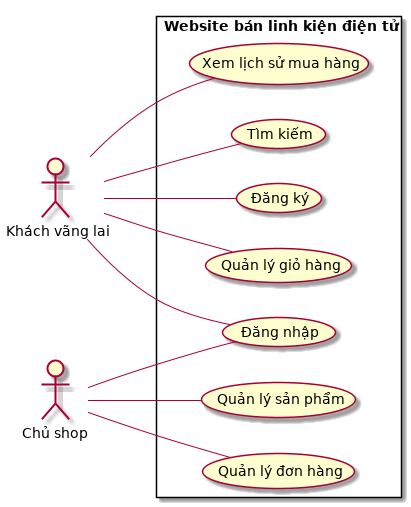
\includegraphics[scale=0.7]{fig/uc_all.png}
        \caption{Biểu đồ tổng quát}
    \end{figure}
\newpage
\item \textbf{Biểu đồ phân rã cho tác nhân Khách hàng}
    \begin{figure}[h!]
        \centering
        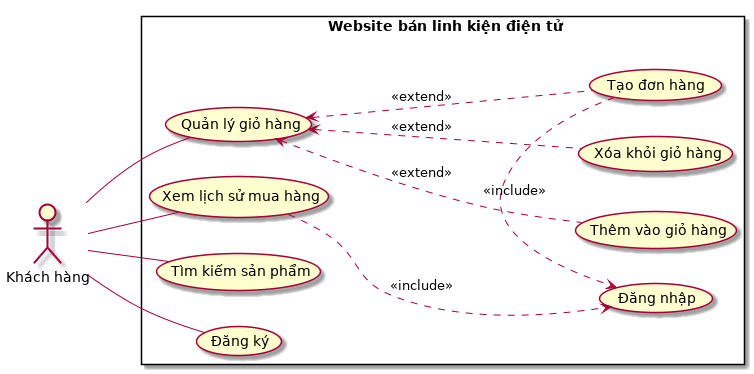
\includegraphics[scale=0.58]{fig/uc_user.png}
        \caption{Biểu đồ phân rã tác nhân Khách hàng}
    \end{figure}
\newpage
\item \textbf{Biểu đồ phân rã cho tác nhân Chủ shop}
    \begin{figure}[h!]
        \centering
        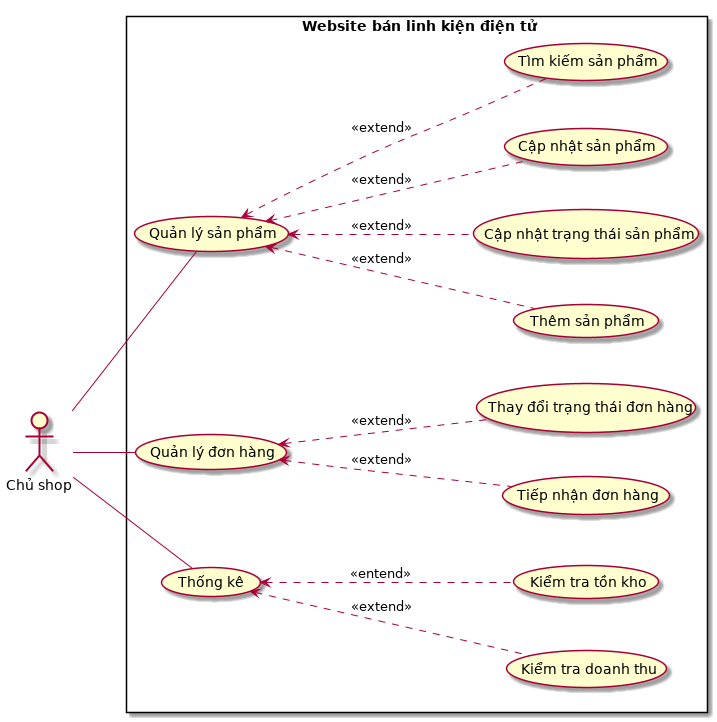
\includegraphics[scale=0.6]{fig/uc_admin.png}
        \caption{Biểu đồ phân rã tác nhân Chủ shop}
    \end{figure}
\end{enumerate}
\subsection{Kịch bản cho một số use case chính}
\begin{center}
\begin{tabularx}{\linewidth}{|X|}
\cline{1-2}
    \textbf{Use case 1:} Đăng nhập\\
    \textbf{Tác nhân chính:} Khách vãng lai\\
    \textbf{Mức:} 1\\
    \textbf{Tiền điều kiện:} Không có\\
    \textbf{Luồng kịch bản chính:}\\
    \begin{enumerate}
        \vspace{-2em}
        \itemsep-0.5em
        \item Khách vãng lai nhập tài khoản và mật khẩu của mình và bấm đăng nhập.
        \item Khách vãng lai nhấn nút đăng nhập
        \item Hệ thống xác thực thông tin Khách vãng lai nhập vào.
        \item Hệ thống tiến hàng đăng nhập
        \item Hệ thống điều hướng và đưa người dùng về trang quản lý phù hợp với từng loại tài khoản (Trang quản lý thông tin cá nhân đối với Người dùng thông thường, trang quản lý đối với chủ cửa hàng).
        \vspace{-1em}
    \end{enumerate}
    \textbf{Ngoại lệ:}\\
    \hspace{1em}2.a: Thông tin khách vãng lai nhập vào không chính xác\\
    \hspace{2.5em}.1 Khách vãng lai có thể chọn đăng ký tài khoản\\
    \textbf{Đảm bảo thành công:} Khách vãng lai đăng nhập thành công và được coi là Người dùng\\
    \textbf{Kích hoạt:} Khách vãng lai chọn chức năng đăng nhập
\cline{1-2}
\end{tabularx}
\end{center}

\begin{center}
\begin{tabularx}{\linewidth}{|X|}
\cline{1-2}
    \textbf{Use case 2:} Đăng ký\\
    \textbf{Tác nhân chính:} Khách vãng lai\\
    \textbf{Mức:} 1\\
    \textbf{Tiền điều kiện:} Không có\\
    \textbf{Luồng kịch bản chính:}\\
    \begin{enumerate}
        \vspace{-2em}
        \itemsep-0.5em
        \item Khách vãng lai nhập những thông tin được yêu cầu vào form đăng ký 
        \item Khách vãng lai nhấn nút đăng ký
        \item Hệ thống xác thực thông tin Khách vãng lai nhập vào.
        \item Hệ thống điều hướng và đưa người dùng về trang đăng nhập.
        \vspace{-1em}
    \end{enumerate}
    \textbf{Ngoại lệ:}\\
    \hspace{1em}2.a: Khách vãng lai nhập thiếu thông tin hoặc thông tin nhập vào không hợp lệ\\
    \hspace{2.5em}.1 Hệ thống yêu cầu người dùng nhập lại thông tin\\
    \textbf{Đảm bảo thành công:} Khách vãng lai đăng nhập thành công và được coi là Người dùng\\
    \textbf{Kích hoạt:} Khách vãng lai chọn chức năng đăng ký
\cline{1-2}
\end{tabularx}
\end{center}

\begin{center}
\begin{tabularx}{\linewidth}{|X|}
\cline{1-2}
    \textbf{Use case 3:} Thêm sản phẩm vào giỏ hàng\\
    \textbf{Tác nhân chính:} Người dùng\\
    \textbf{Mức:} 3\\
    \textbf{Tiền điều kiện:} Đã thực hiện usecase 1 và là người dùng thông thường\\
    \textbf{Luồng kịch bản chính:}\\
    \begin{enumerate}
        \vspace{-2em}
        \itemsep-0.5em
        \item Người dùng tìm kiếm và chọn ra sản phẩm mà mình mong muốn
        \item Người dùng chọn xem chi tiết sản phẩm và chọn số lượng sản phẩm muốn mua sau đó bấm thêm vào giỏ hàng
        \item Hệ thống thực hiện thêm thông tin sản phẩm  (id, số lượng, đơn giá) vào giỏ hàng
        \item Hệ thống cập nhật số sản phẩm trong giỏ hàng
        \vspace{-1em}
    \end{enumerate}
    \textbf{Ngoại lệ:}\\
    \hspace{1em}2.a: Sản phẩm hết hàng hoặc ngừng kinh doanh\\
    \hspace{2.5em}.1 Hệ thống ẩn nút Thêm vào giỏ hàng và hiện thông báo với người dùng\\
    \hspace{1em}3.a: Sản phẩm hết hàng hoặc ngừng kinh doanh\\
    \hspace{2.5em}.1 Nếu sản phẩm đã được thêm từ trước thì hệ thống sẽ chỉ tăng số lượng sản phẩm\\
    \textbf{Đảm bảo thành công:} Thông tin sản phẩm được cập nhật thành công\\
    \textbf{Kích hoạt:} Chủ cửa hàng chọn chức năng quản lý sản phẩm
\cline{1-2}
\end{tabularx}
\end{center}

\begin{center}
\begin{tabularx}{\linewidth}{|X|}
\cline{1-2}
    \textbf{Use case 4:} Tạo hóa đơn\\
    \textbf{Tác nhân chính:} Không có\\
    \textbf{Mức:} 3\\
    \textbf{Tiền điều kiện:} Có ít nhất một sản phẩm trong giỏ hàng\\
    \textbf{Luồng kịch bản chính:}\\
    \begin{enumerate}
        \vspace{-2em}
        \itemsep-0.5em
        \item Hệ thống kiểm tra, nếu là khách vãng lai thì yêu cầu đăng nhập
        \item Người dùng thay đổi địa chỉ ship hàng và thêm ghi chú (nếu cần) sau đó bấm đặt hàng
        \item Hệ thống thêm đơn hàng vào CSDL và đưa ra thông báo đặt hàng thành công
        \vspace{-1em}
    \end{enumerate}
    \textbf{Ngoại lệ:}\\
    \hspace{1em}2.a: Địa chỉ ship để trống\\
    \hspace{2.5em}.1 Hệ thống thông báo lỗi tới người dùng\\
    \textbf{Đảm bảo thành công:} Thông tin sản phẩm được cập nhật thành công\\
    \textbf{Kích hoạt:} Chủ cửa hàng chọn chức năng quản lý sản phẩm
\cline{1-2}
\end{tabularx}
\end{center}

\begin{center}
\begin{tabularx}{\linewidth}{|X|}
\cline{1-2}
    \textbf{Use case 5:} Cập nhật thông tin sản phẩm\\
    \textbf{Tác nhân chính:} Chủ cửa hàng\\
    \textbf{Mức:} 3\\
    \textbf{Tiền điều kiện:} Đã đăng nhập vào hệ thống với tài khoản quản trị\\
    \textbf{Luồng kịch bản chính:}\\
    \begin{enumerate}
        \vspace{-2em}
        \itemsep-0.5em
        \item Chủ cửa hàng tìm kiếm sản phầm muốn sửa hoặc chọn tại danh sách mới thêm và bấm sửa
        \item Chủ cửa hàng nhập thông tin mới cập nhật
        \item Chủ cửa hàng bấm nút đăng nhập
        \item Hệ thống kiểm tra thông tin người dùng nhập vào và cập nhật Lên CSDL
        \item Hệ thống điều hướng và đưa người dùng về trang Quản lý thông tin.
        \vspace{-1em}
    \end{enumerate}
    \textbf{Ngoại lệ:}\\
    \hspace{1em}6.a: Thông tin Chủ cửa hàng nhập vào không hợp lệ\\
    \hspace{2.5em}.1 Hệ thống báo lỗi và không cập nhật thông tin lên CSDL\\
    \textbf{Đảm bảo thành công:} Thông tin sản phẩm được cập nhật thành công\\
    \textbf{Kích hoạt:} Chủ cửa hàng chọn chức năng quản lý sản phẩm
\cline{1-2}
\end{tabularx}
\end{center}
\newpage
\subsection{Biểu đồ lớp}
\begin{figure}[h!]
    \centering
    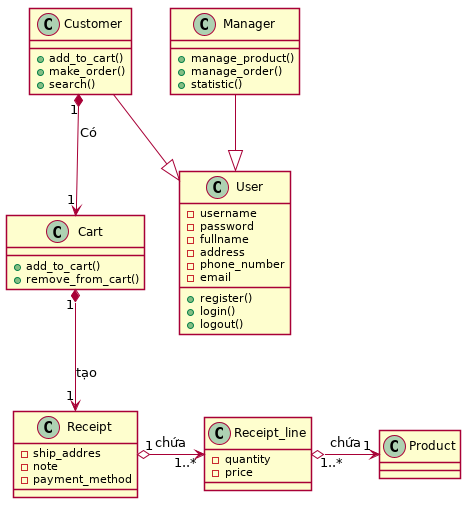
\includegraphics[scale=0.7]{fig/class.png}
    \caption{Biểu đồ lớp}
\end{figure}
\newpage
\subsection{Biểu đồ hoạt động}
\begin{enumerate}[label=\textbf{\alph*)}]
    \item Biểu đồ hoạt động cho chức năng đăng nhập
    \begin{figure}[h!]
       \centering
       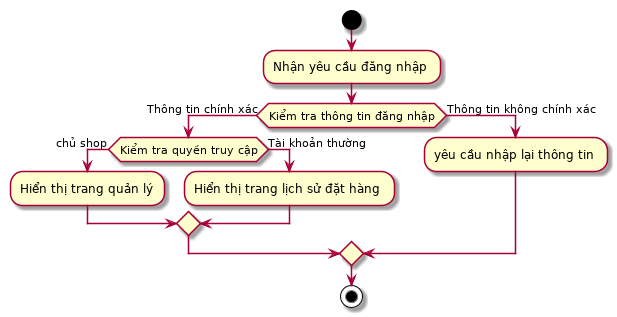
\includegraphics[scale=0.7]{fig/a_login.png}
       \caption{Biểu đồ hoạt động cho chức năng đăng nhập}
    \end{figure}
    \item Biểu đồ hoạt động cho chức năng thêm vào giỏ hàng
    \begin{figure}[h!]
       \centering
       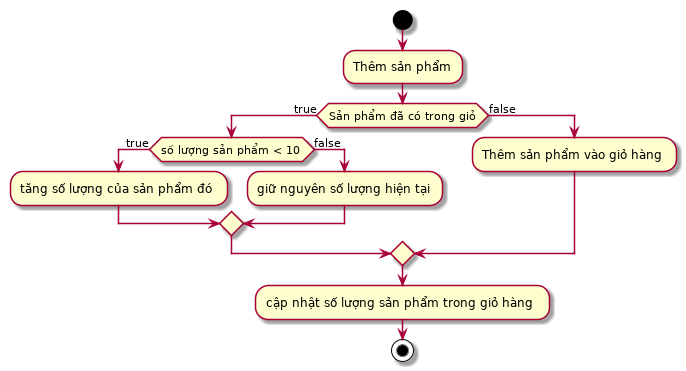
\includegraphics[scale=0.7]{fig/a_cart.png}
       \caption{Biểu đồ hoạt động cho chức năng thêm vào giỏ hàng}
    \end{figure}
    \item Biểu đồ hoạt động cho chức năng thanh toán
    \begin{figure}[h!]
       \centering
       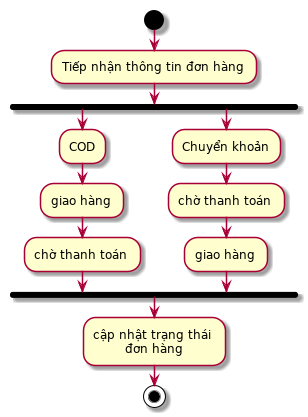
\includegraphics[scale=0.7]{fig/a_order.png}
       \caption{Biểu đồ hoạt động cho chức năng thanh toán}
    \end{figure}
\end{enumerate}
\subsection{Biểu đồ tuần tự cho một số chức năng chính}
\begin{enumerate}[label=\textbf{\alph*)}]
    \item Chức năng lấy thông tin sản phẩm
    \begin{figure}[h!]
        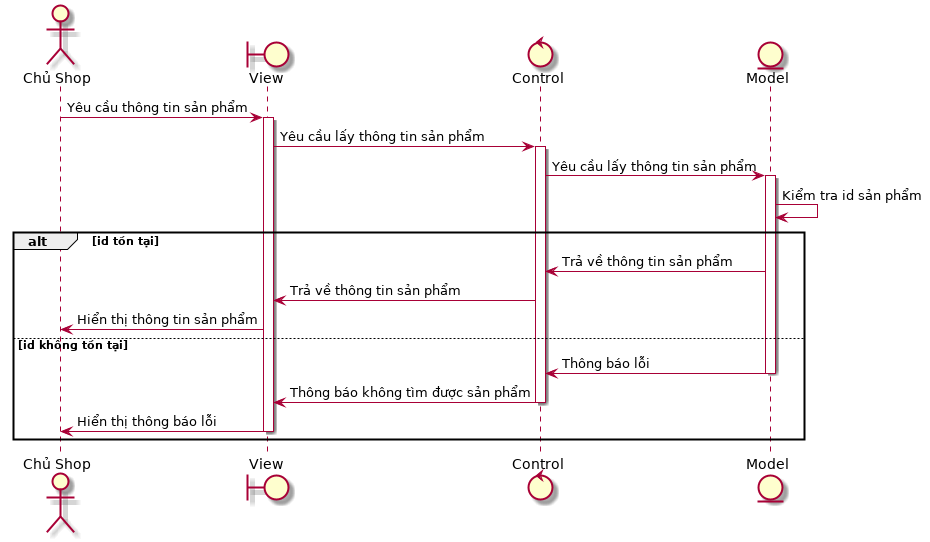
\includegraphics[scale=0.5]{fig/s_get_product_info.png}
        \caption{Biểu đồ tuần tự cho chức năng lấy thông tin sản phẩm}
    \end{figure}

    \item Chức năng cập nhật thông tin sản phẩm
    \begin{figure}[h!]
        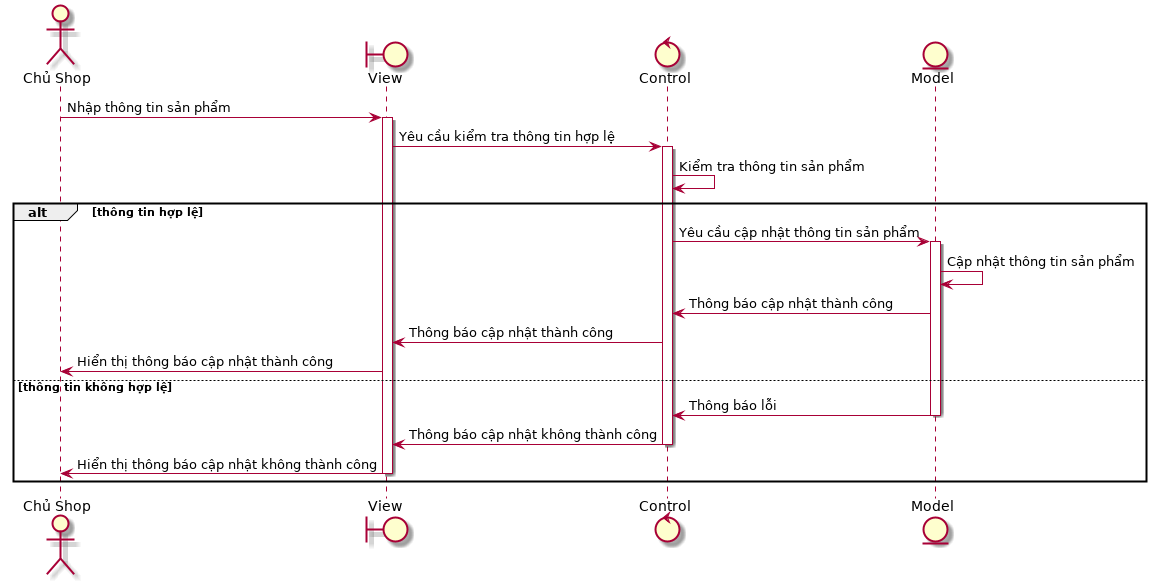
\includegraphics[scale=0.4]{fig/s_update_product_info.png}
        \caption{Biểu đồ tuần tự cho chức năng cập nhật thông tin sản phẩm}
    \end{figure}
    \item Chức năng thêm vào giỏ hàng
    \begin{figure}[h!]
        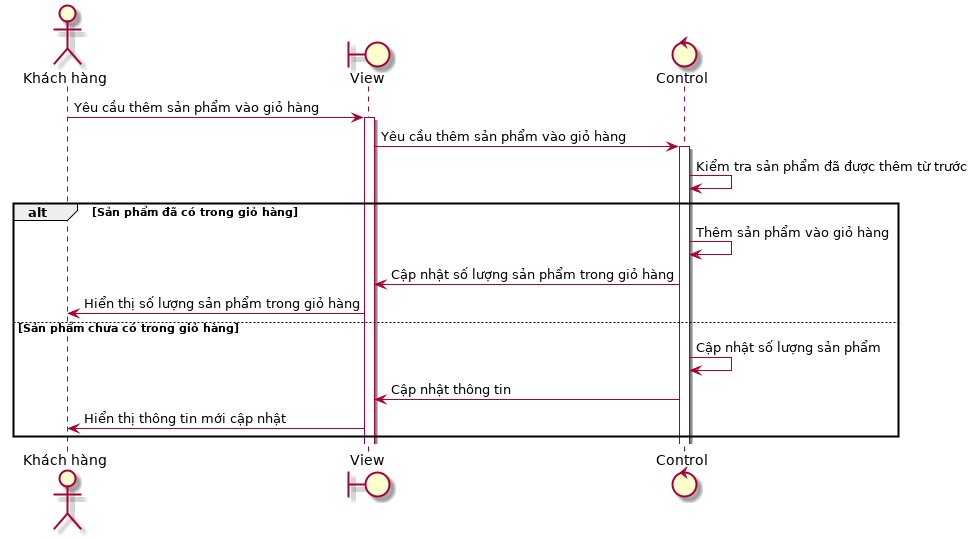
\includegraphics[scale=0.45]{fig/s_add_to_cart.png}
        \caption{Biểu đồ tuần tự cho chức năng thêm vào giỏ hàng}
    \end{figure}
\end{enumerate}
\newpage
\subsection{Biểu đồ quan hệ thực thể}
\begin{figure}[h!]
    \centering
    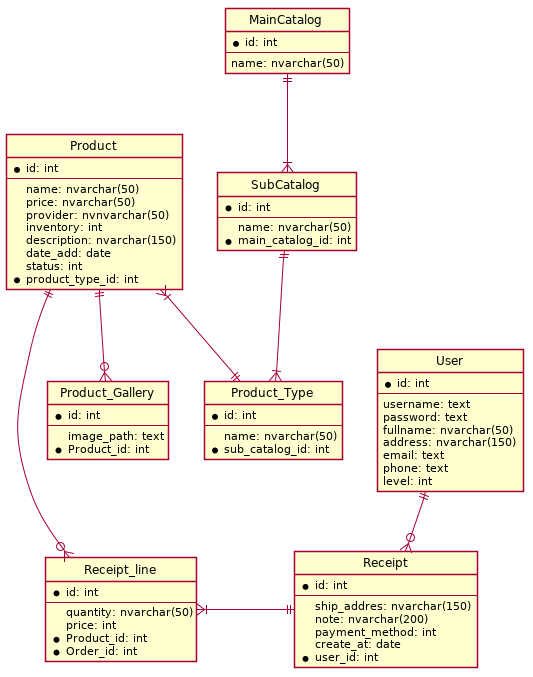
\includegraphics[scale=0.6]{fig/er.png}
    \caption{Biểu đồ quan hệ thực thể}
\end{figure}
\newpage
\subsection{Biểu đồ triển khai}
\begin{figure}[h!]
    \centering
    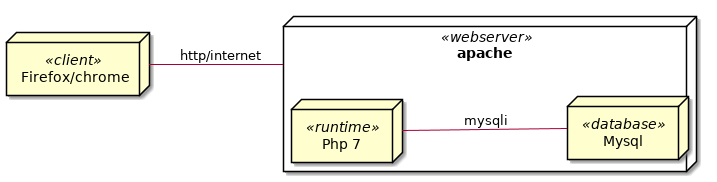
\includegraphics[scale=0.6]{fig/deploy.png}
    \caption{Biểu đồ triển khai}
\end{figure}
\section{Một số nguyên mẫu thiết kế trang web}
\begin{enumerate}[label=\textbf{\alph*)}]
    \item Thiết kế trang chủ
    \begin{figure}[h!]
       \centering
       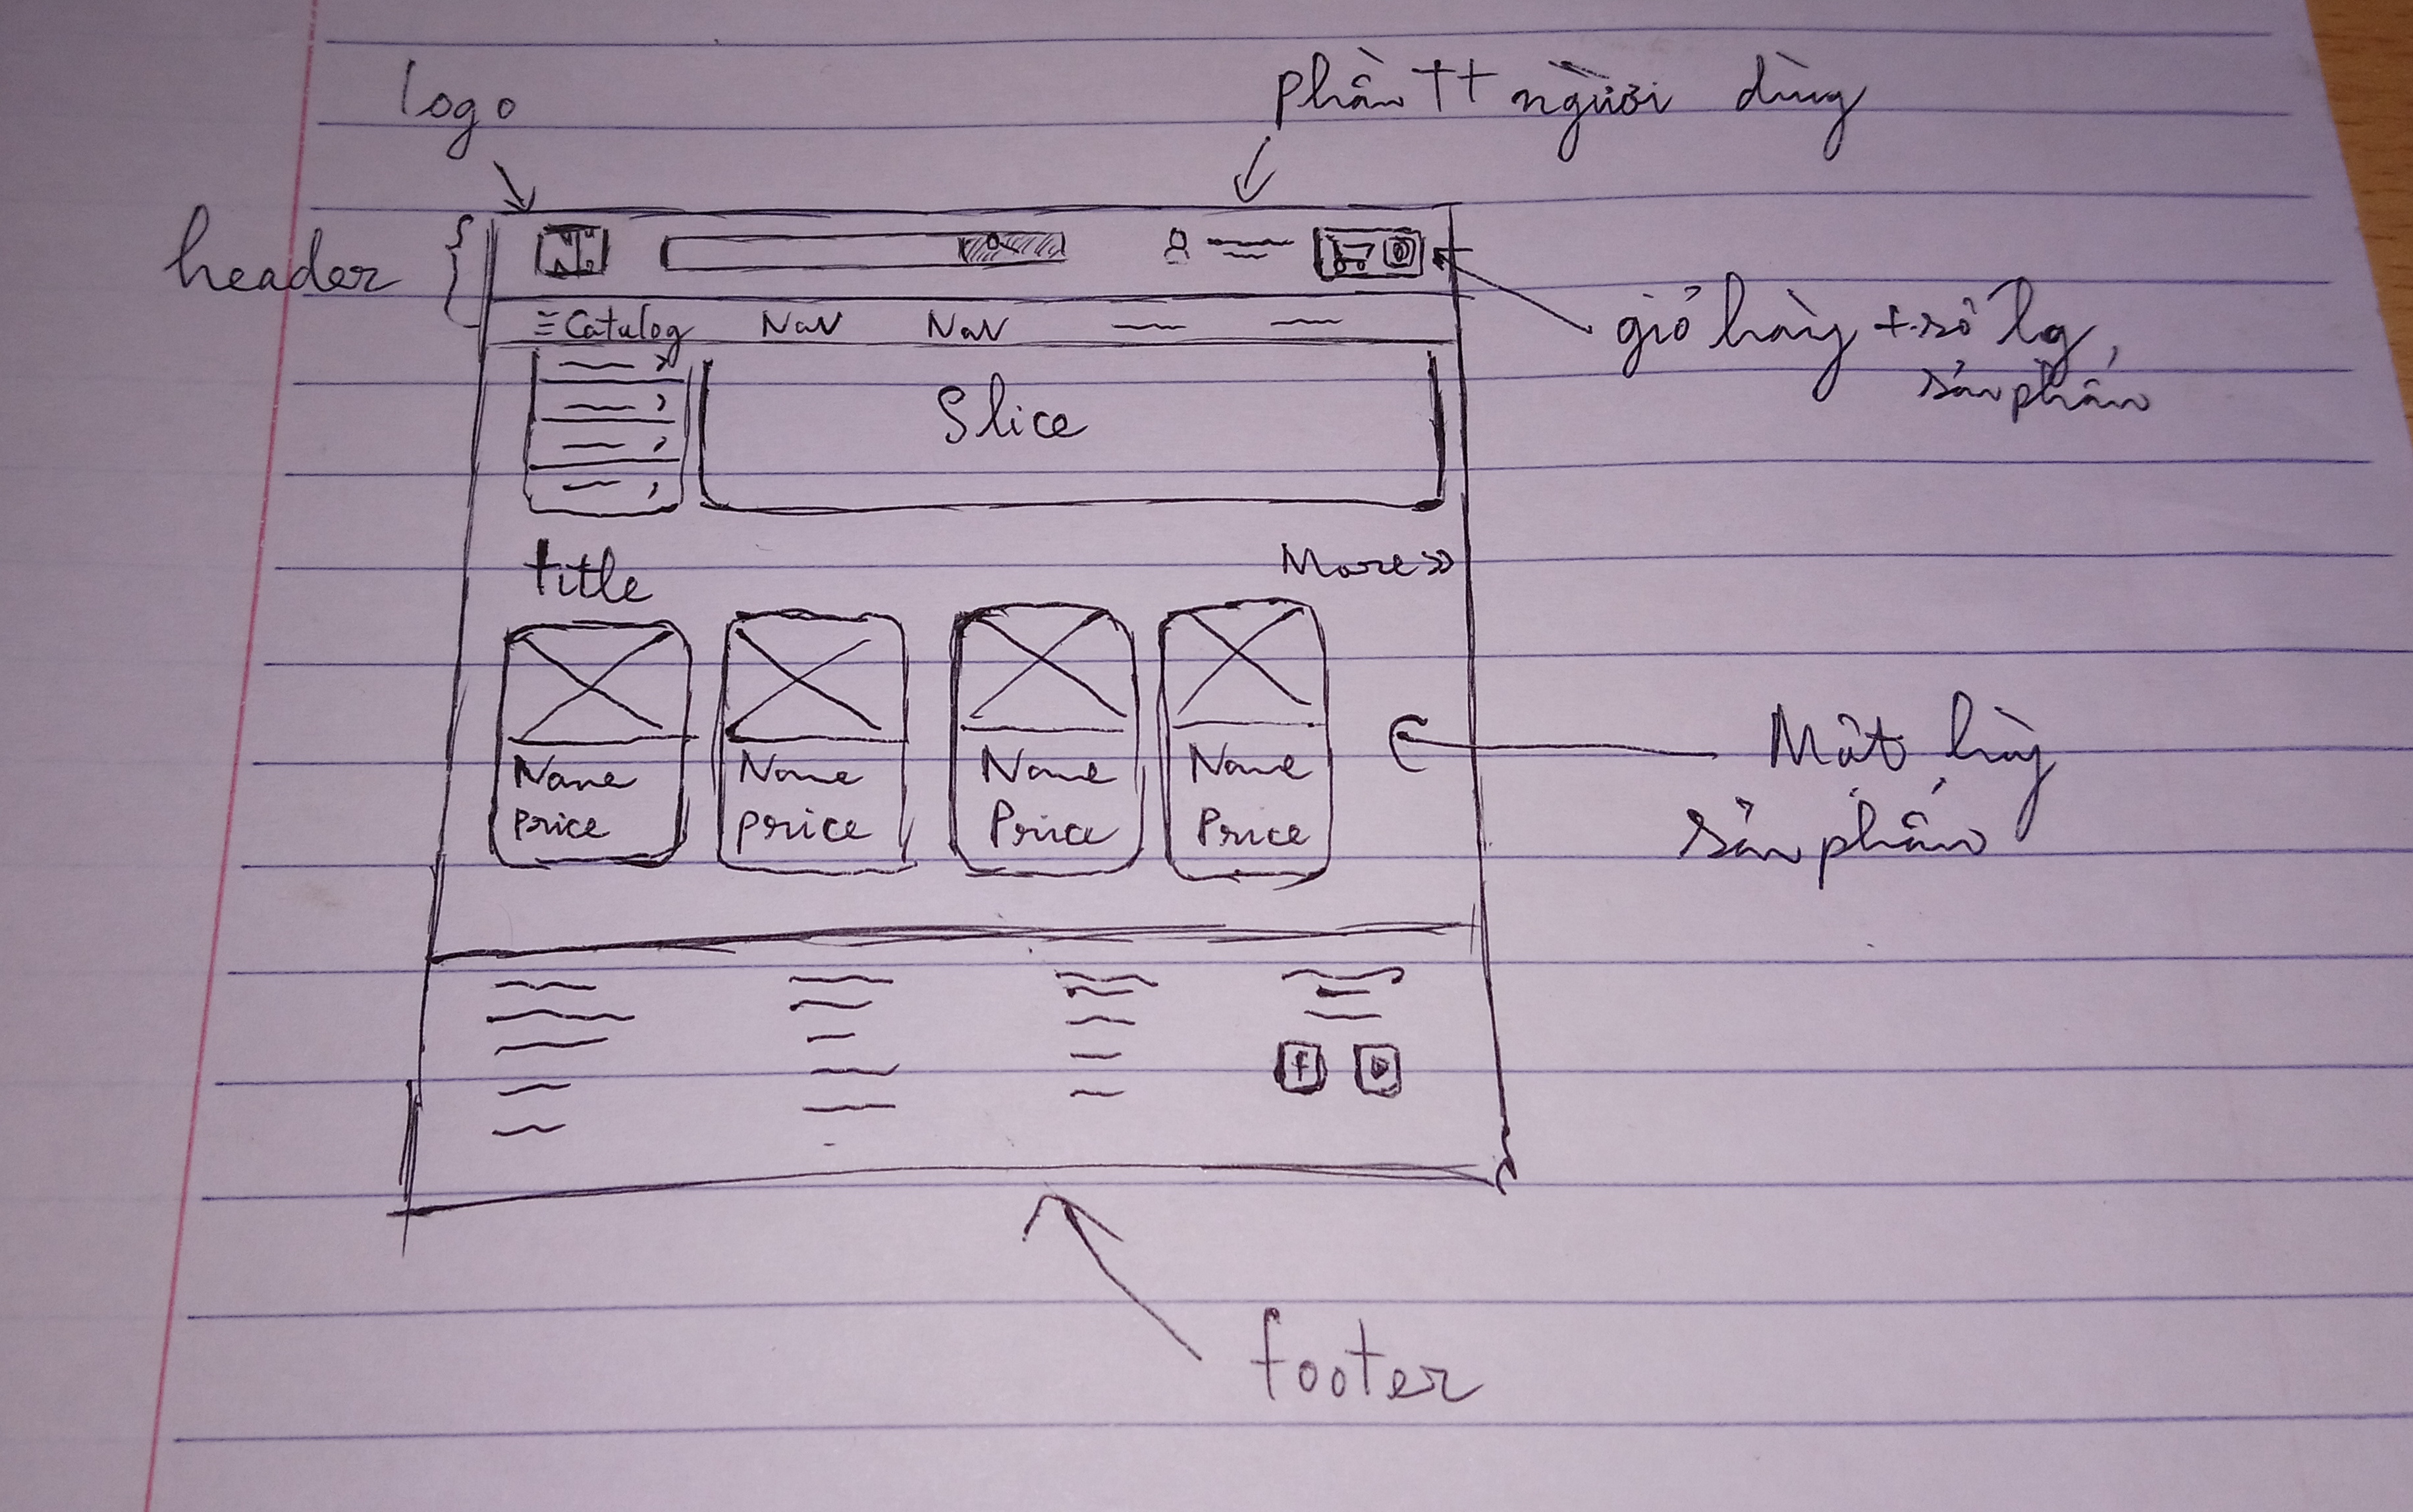
\includegraphics[width=\linewidth]{fig/p_home.jpg}
       \caption{Nguyên mẫu thiết kế trang chủ}
    \end{figure}
    \newpage
    \item Thiết kế giỏ hàng
    \begin{figure}[h!]
       \centering
       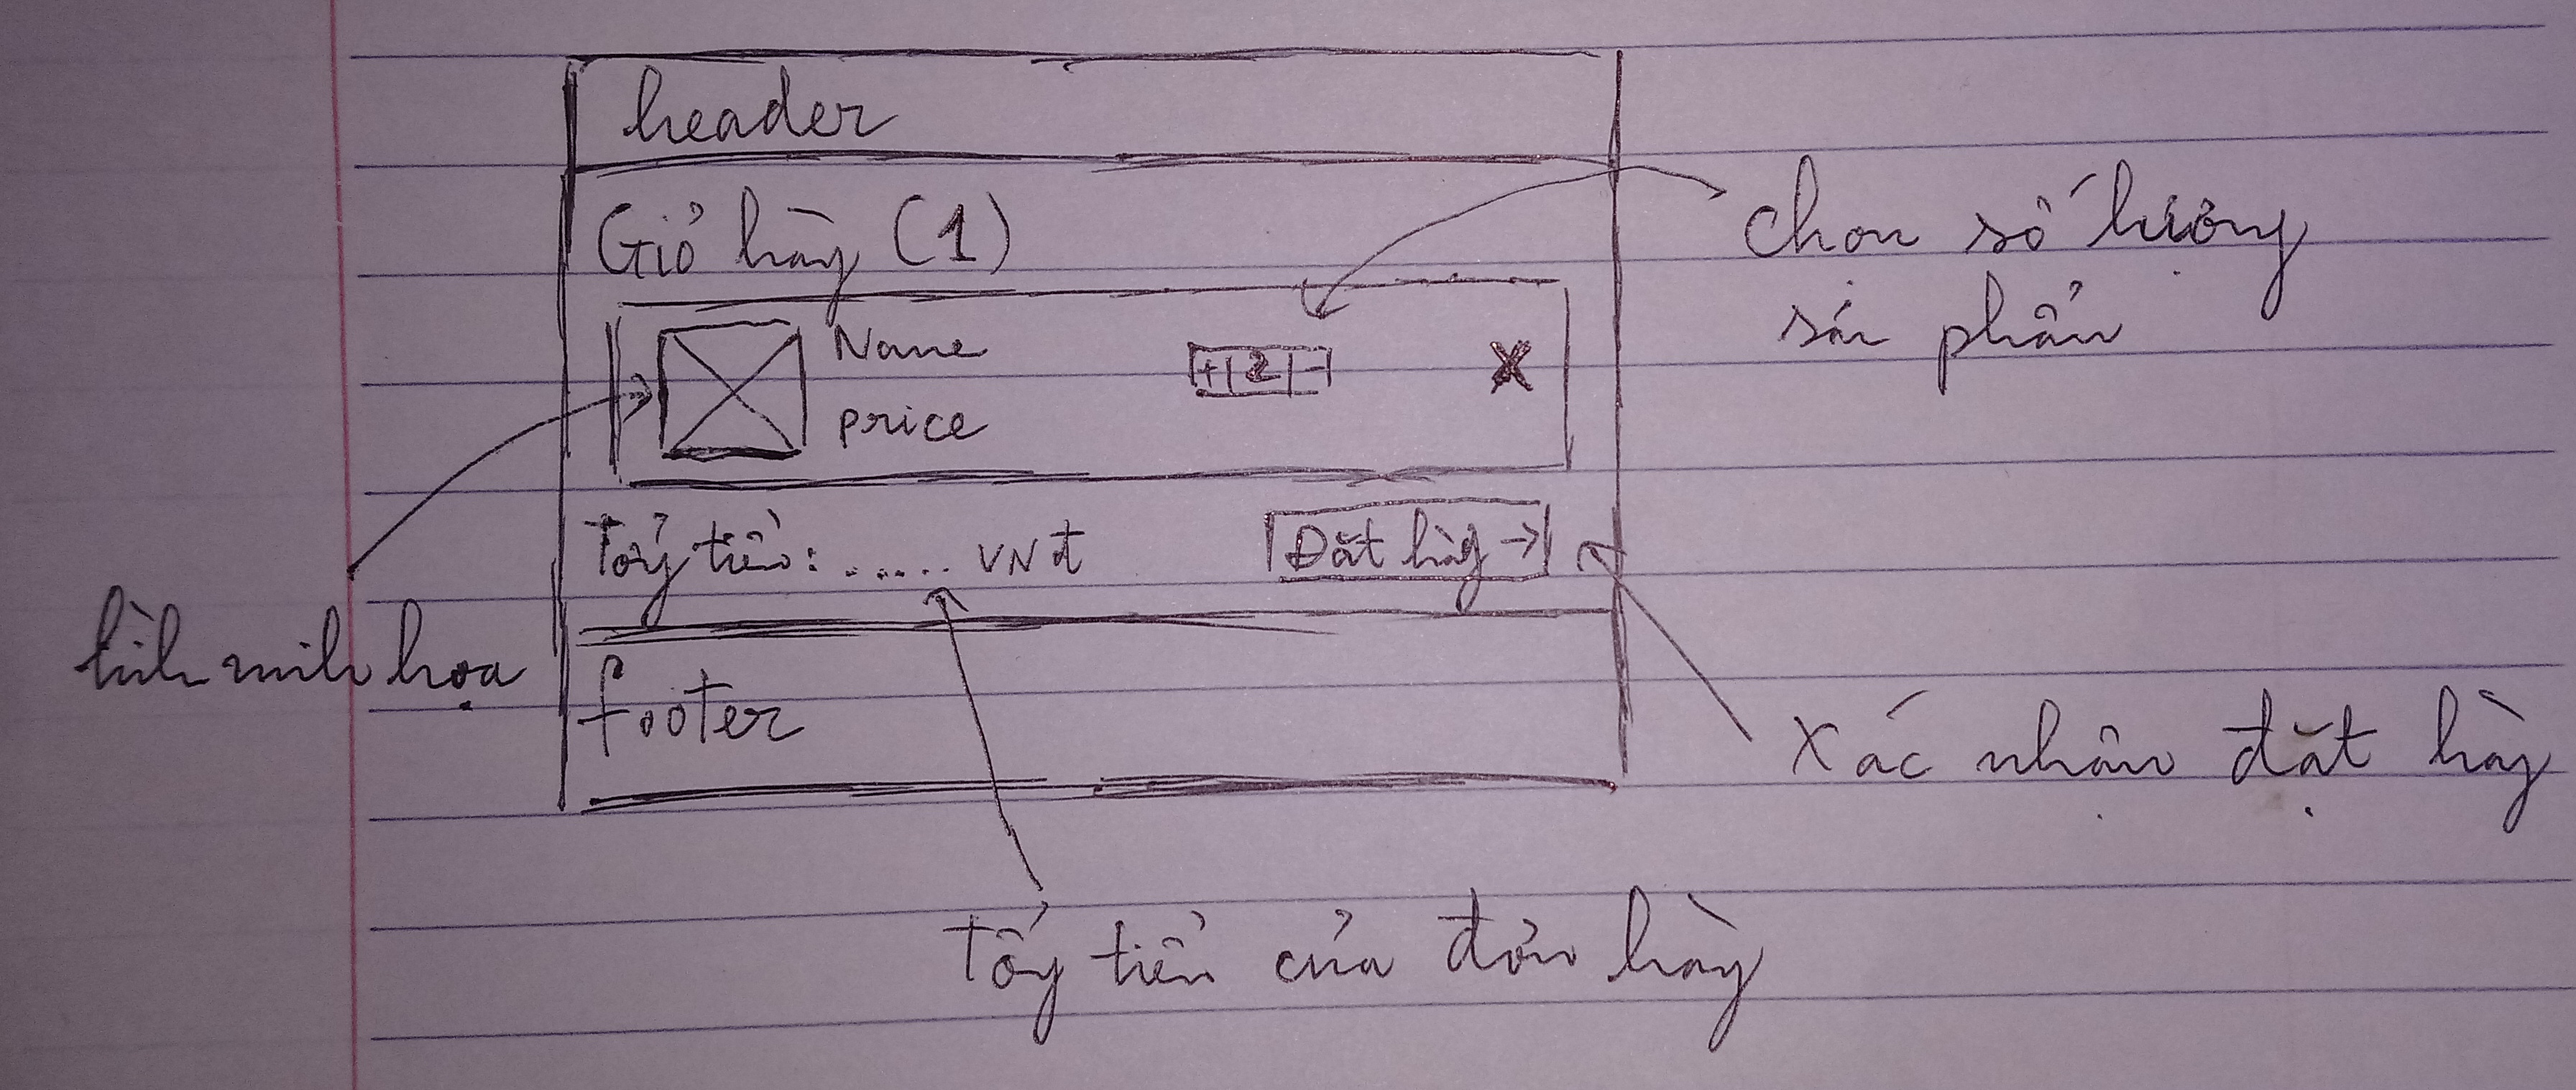
\includegraphics[width=\linewidth]{fig/p_cart.jpg}
       \caption{Nguyên mẫu thiết kế giỏ hàng}
    \end{figure}
    \item Thiết kế trang quản trị
    \begin{figure}[h!]
       \centering
       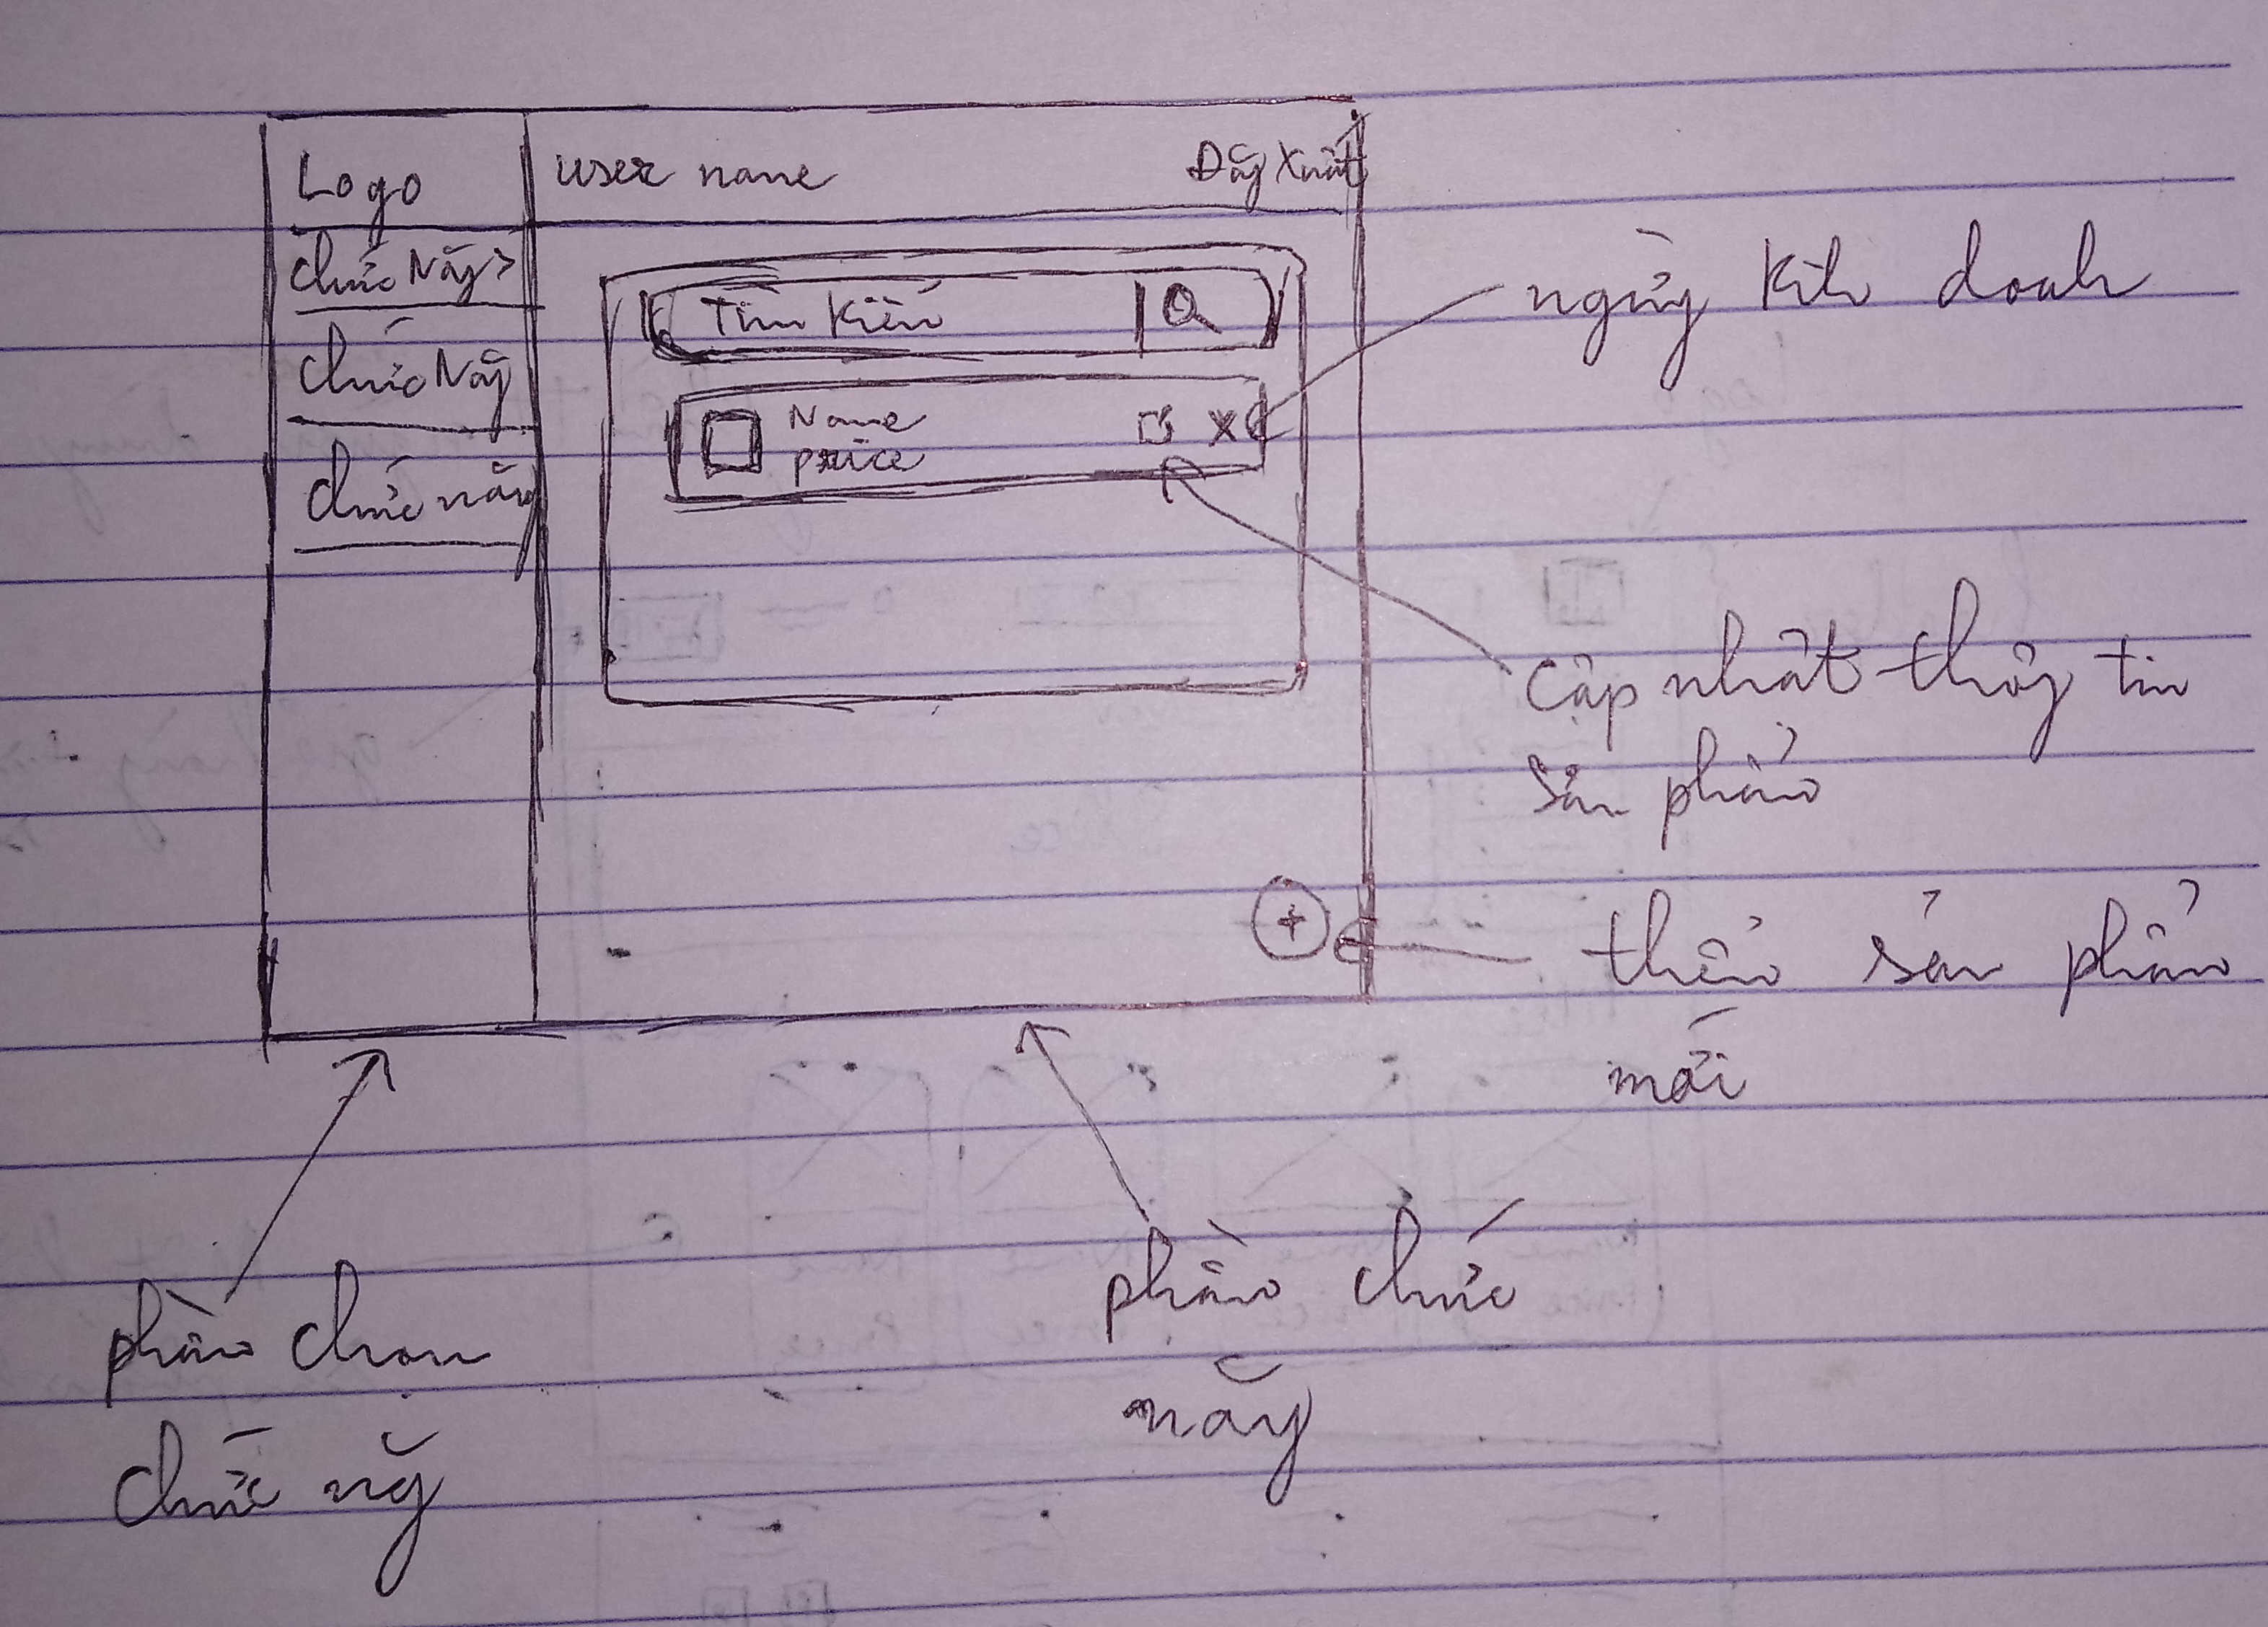
\includegraphics[width=\linewidth]{fig/p_dashboard.jpg}
       \caption{Nguyên mẫu thiết kế trang chủ}
    \end{figure}
\end{figure}
\section{Hình ảnh thực tế}
\begin{enumerate}[label=\textbf{\alph*)}]
    \item Trang chủ
    \begin{figure}[h!]
       \centering
        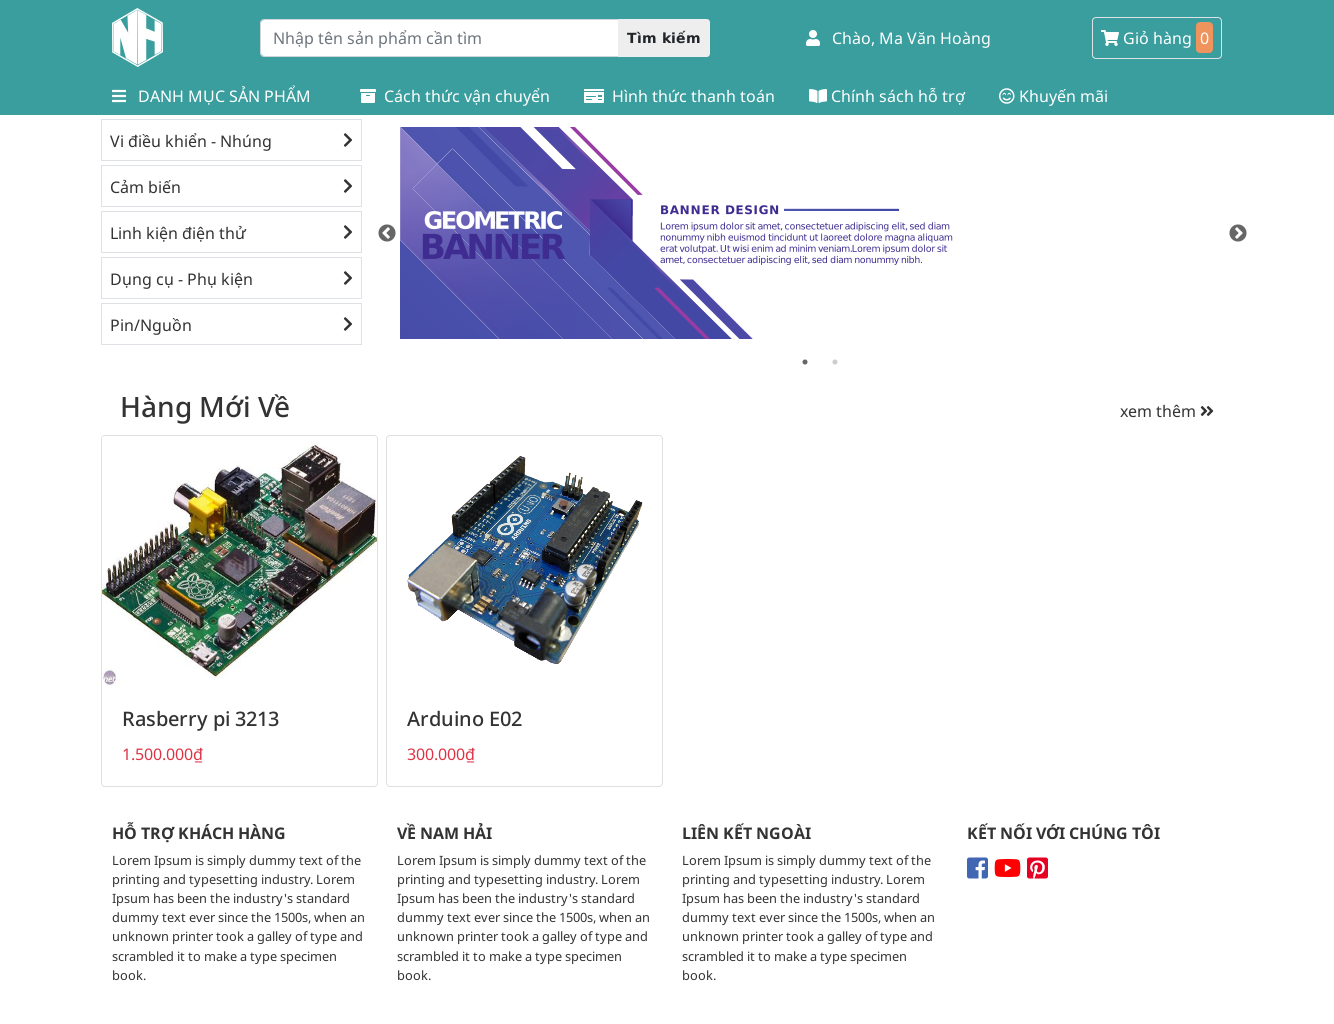
\includegraphics[scale=0.27]{fig/r_home.png}
       \caption{Thiết kế trang chủ}
    \end{figure}
    \item Chi tiết sản phẩm
    \begin{figure}[h!]
       \centering
        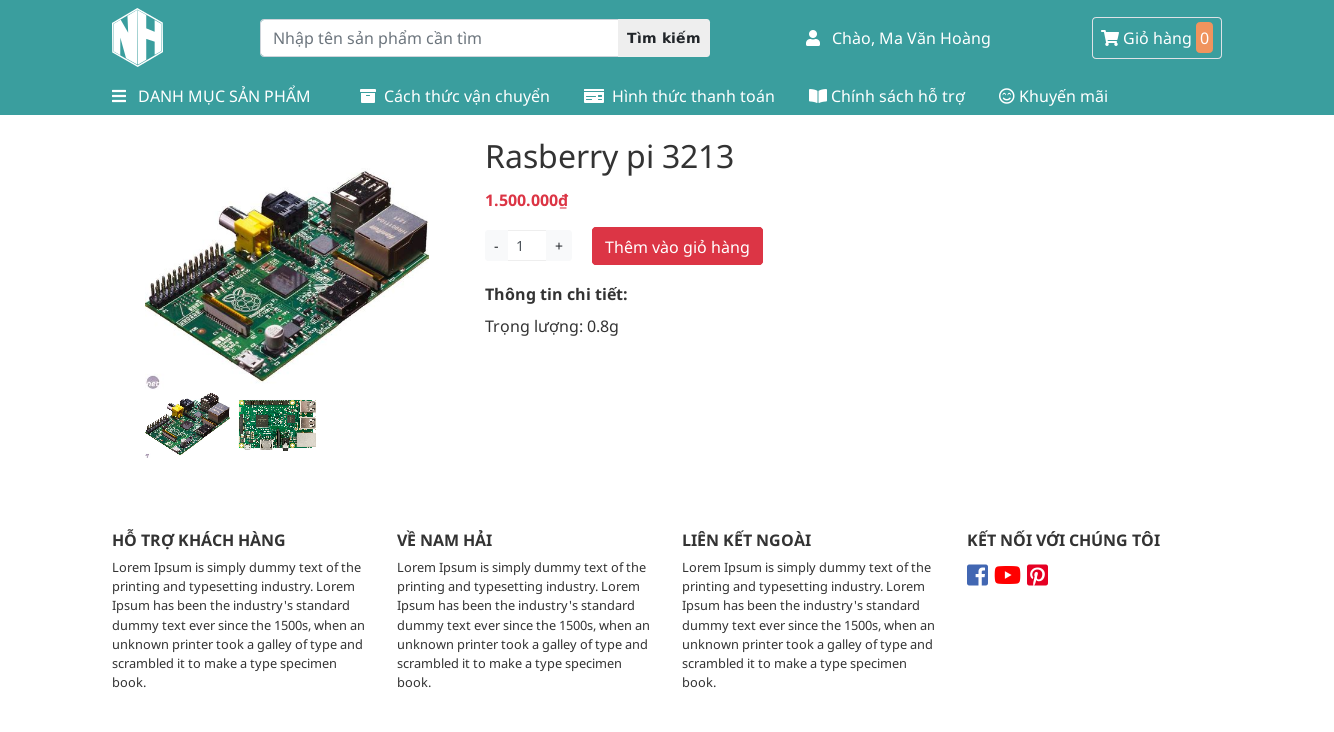
\includegraphics[scale=0.27]{fig/r_product_details.png}
       \caption{Thiết kế trang chi tiết sản phẩm}
    \end{figure}
    \newpage
    \item Giỏ hàng
    \begin{figure}[h!]
       \centering
        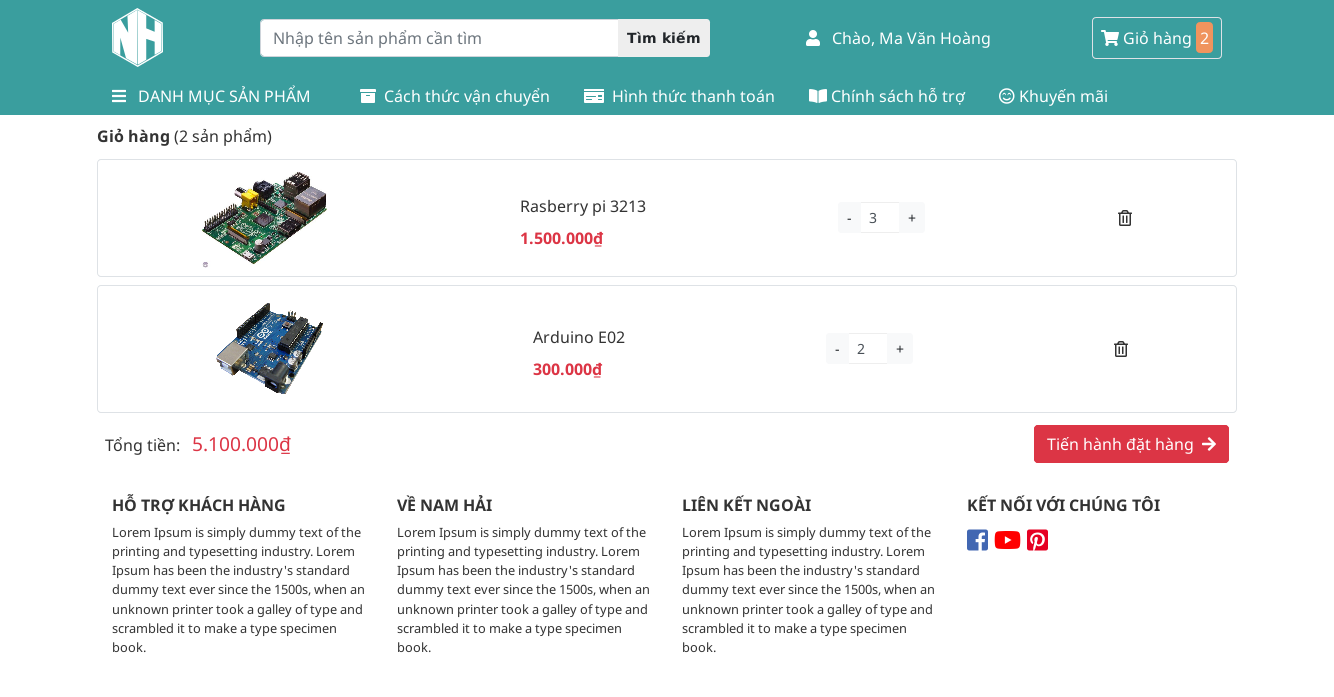
\includegraphics[width=\linewidth]{fig/r_cart.png}
       \caption{Thiết kế trang giỏ hàng}
    \end{figure}
    \item Tạo hóa đơn
    \begin{figure}[h!]
       \centering
        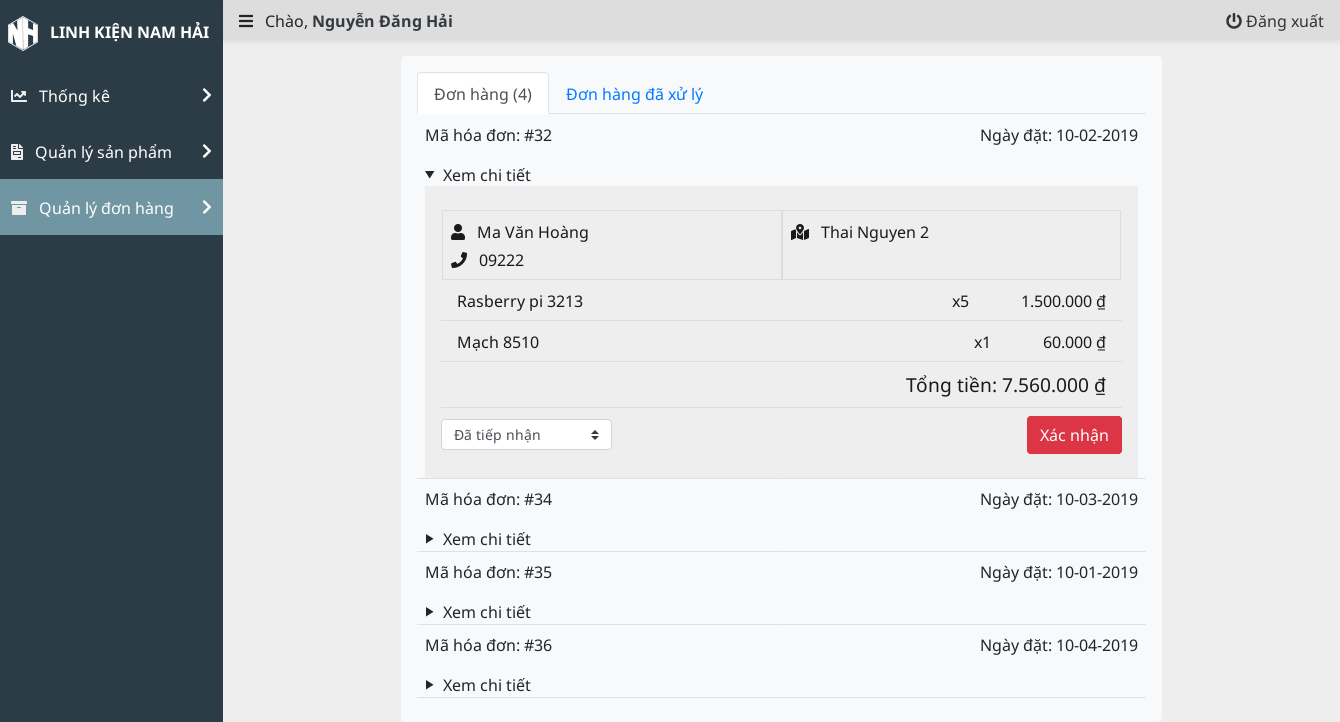
\includegraphics[width=\linewidth]{fig/r_order.png}
       \caption{Thiết kwidth=\linewidthế trang tạo hóa đơn}
    \end{figure}
    \newpage
    \item Lịch sử giao dịch
    \begin{figure}[h!]
       \centering
        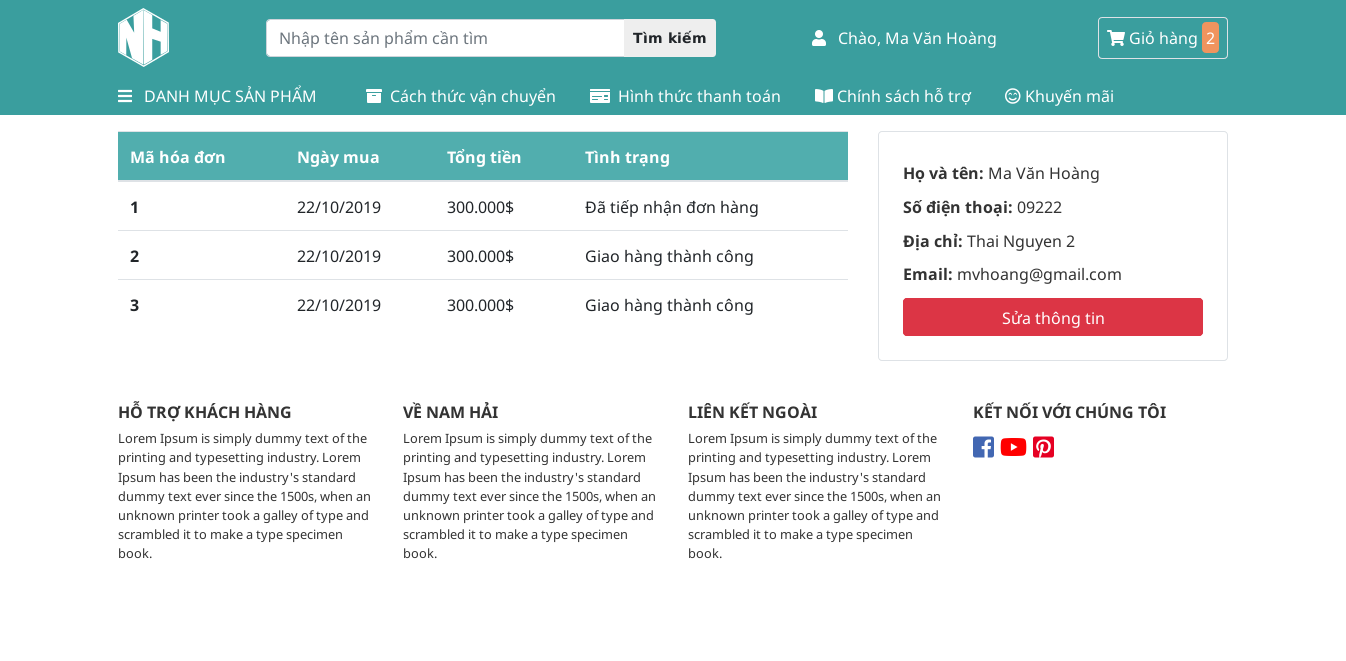
\includegraphics[width=\linewidth]{fig/r_user1.png}
       \caption{Thiết kế trang lịch sử giao dịch}
    \end{figure}
    \item Cập nhật thông tin cá nhân
    \begin{figure}[h!]
       \centering
        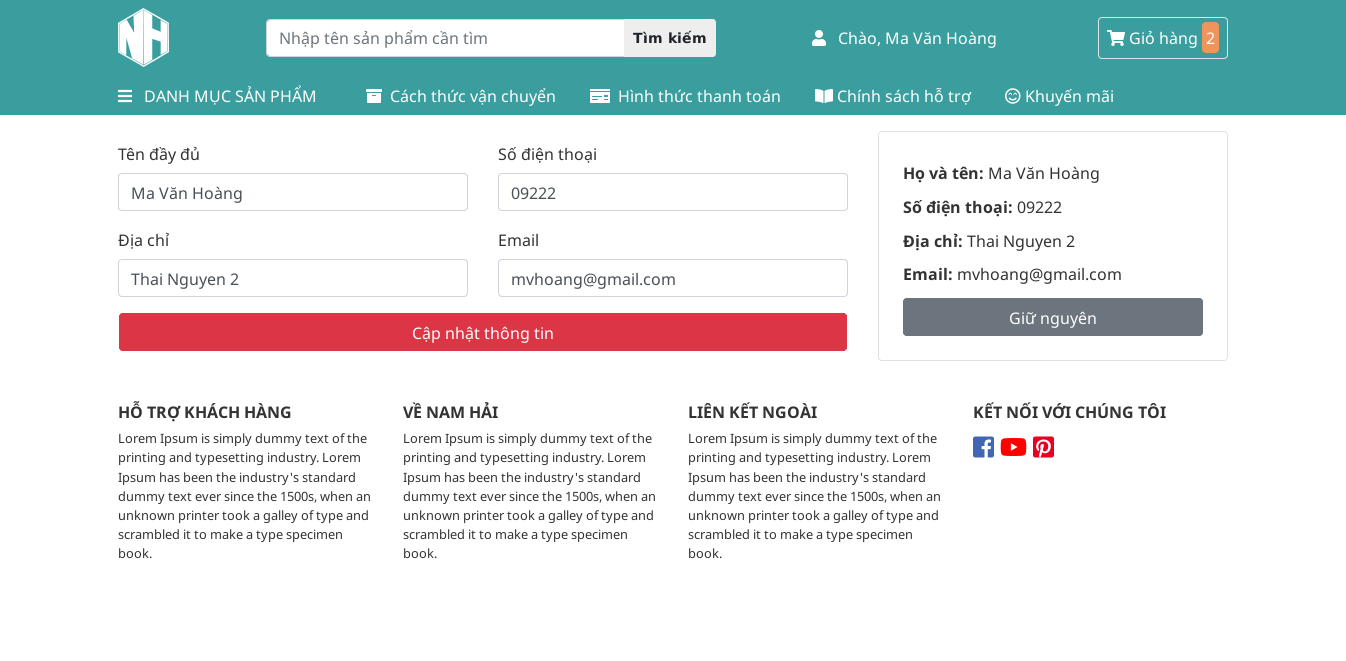
\includegraphics[width=\linewidth]{fig/r_user2.png}
       \caption{Thiết kế trang cập nhật thông tin cá nhân}
    \end{figure}
    \newpage
    \item Trang quản lý
    \begin{figure}[h!]
       \centering
        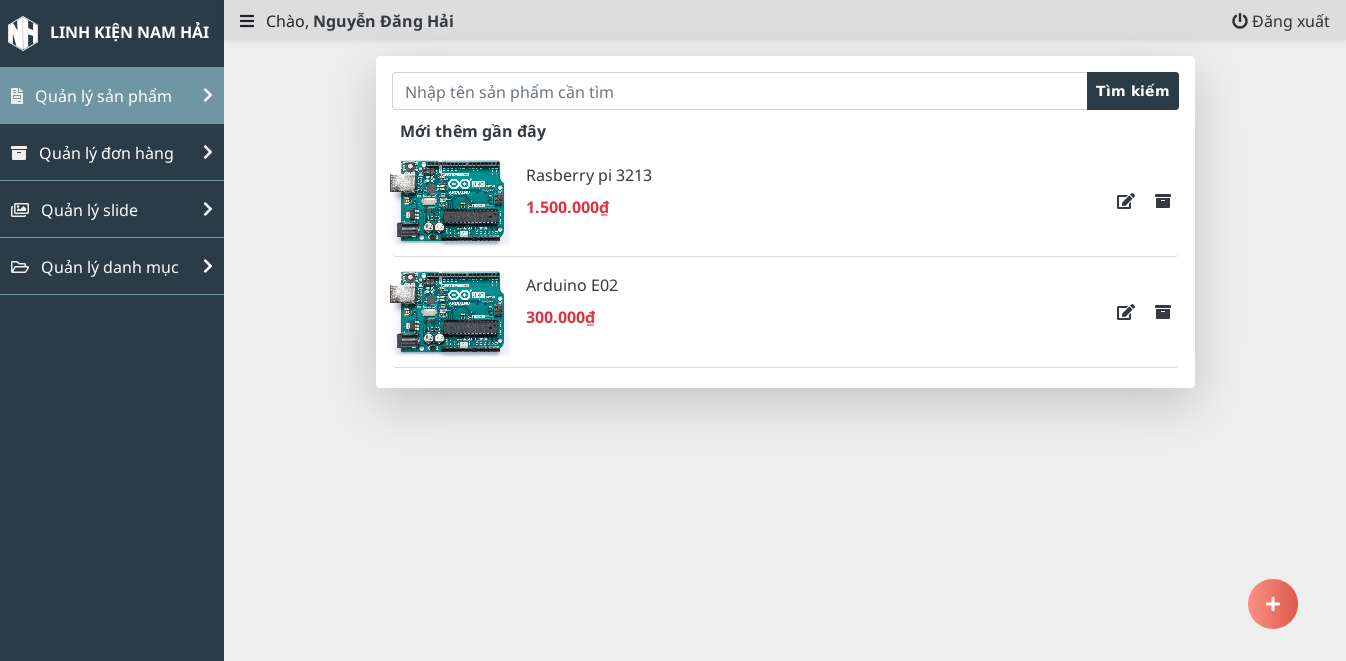
\includegraphics[width=\linewidth]{fig/r_manage_product.png}
       \caption{Thiết kế trang quản lý}
    \end{figure}
    \item Trang thêm sản phẩm
    \begin{figure}[h!]
       \centering
        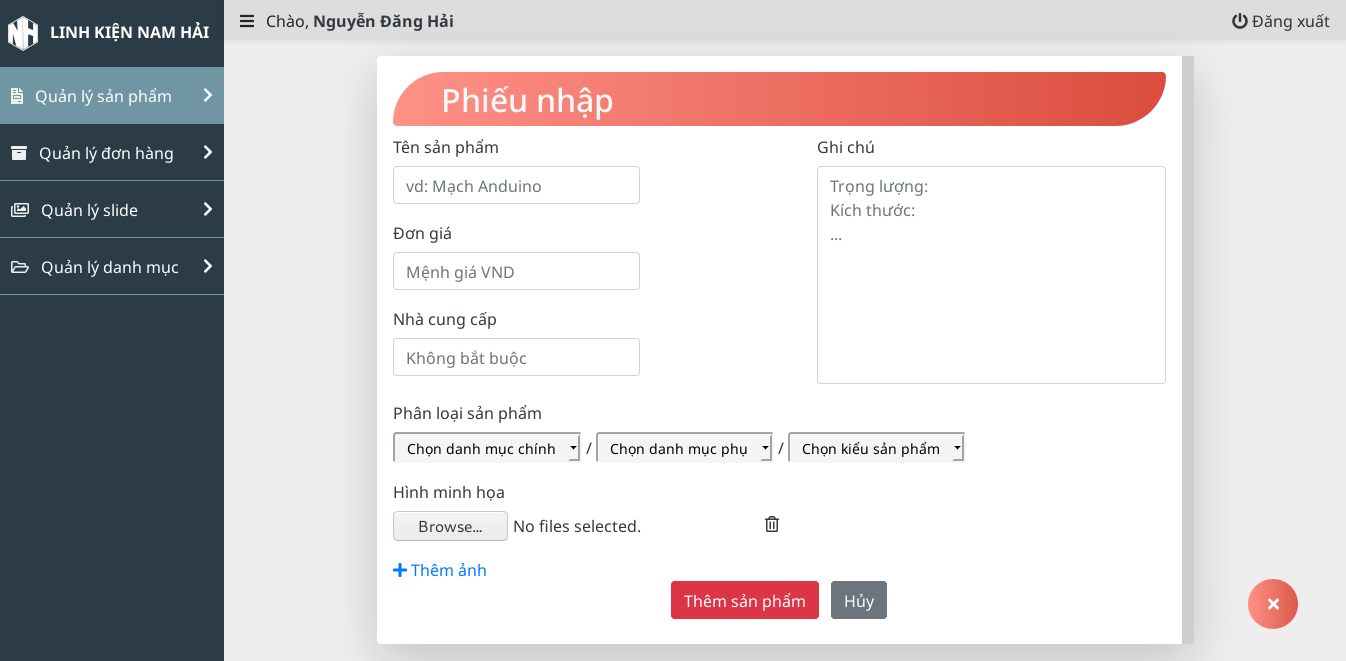
\includegraphics[width=\linewidth]{fig/r_manage_product_add_product.png}
       \caption{Thiết kế trang quản thêm sản phẩm}
    \end{figure}
    \newpage
    \item Trang cập nhật thông tin sản phẩm
    \begin{figure}[h!]
       \centering
        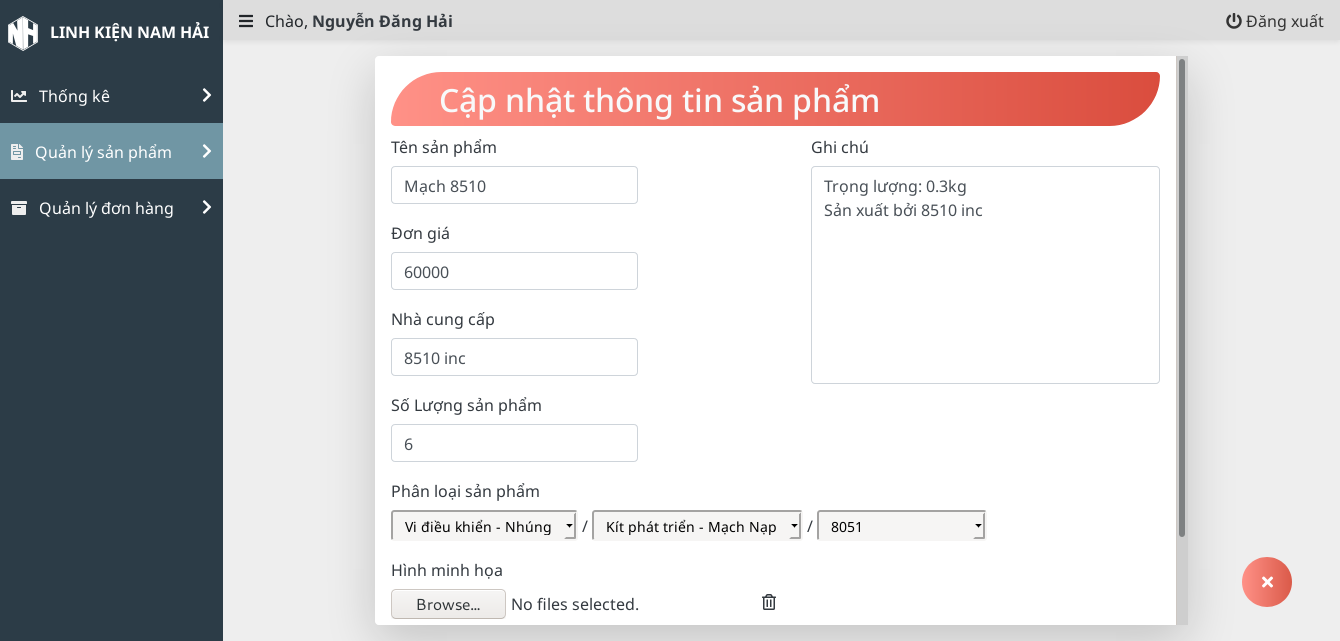
\includegraphics[width=\linewidth]{fig/r_manage_product_update_product.png}
       \caption{Thiết kế trang cập nhật thông tin sản phẩm}
    \end{figure}
\end{enumerate}

\chapter{Cài đặt chương trình}
\section{Hình ảnh thực tế}
\begin{enumerate}[label=\textbf{\alph*)}]
	\item Trang chủ
	      \begin{figure}[h!]
		      \centering
		      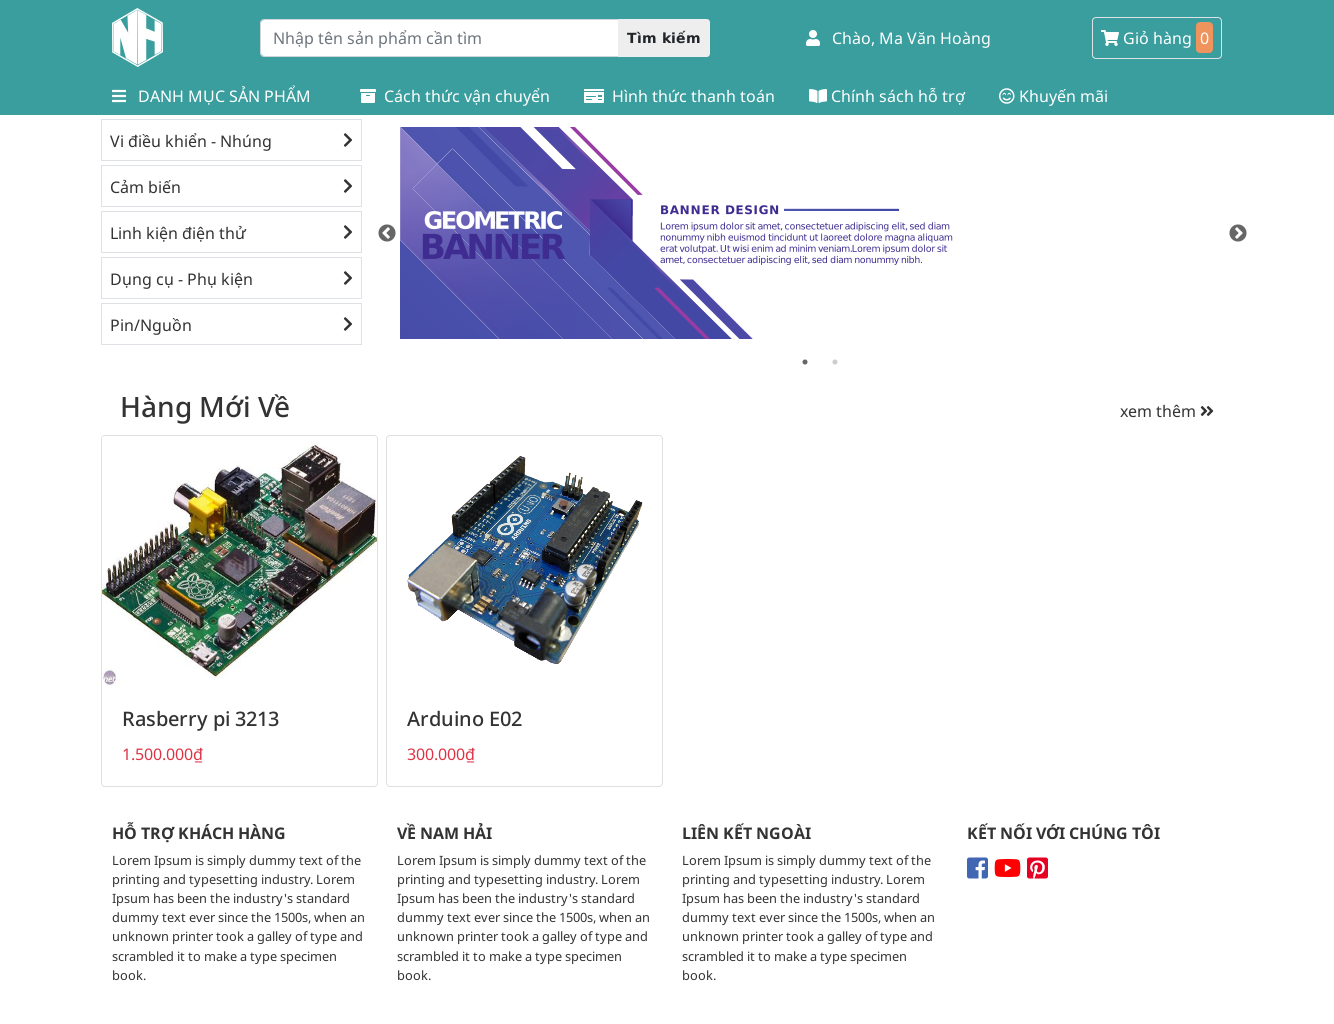
\includegraphics[scale=0.27]{fig/r_home.png}
		      \caption{Thiết kế trang chủ}
	      \end{figure}
	\item Chi tiết sản phẩm
	      \begin{figure}[h!]
		      \centering
		      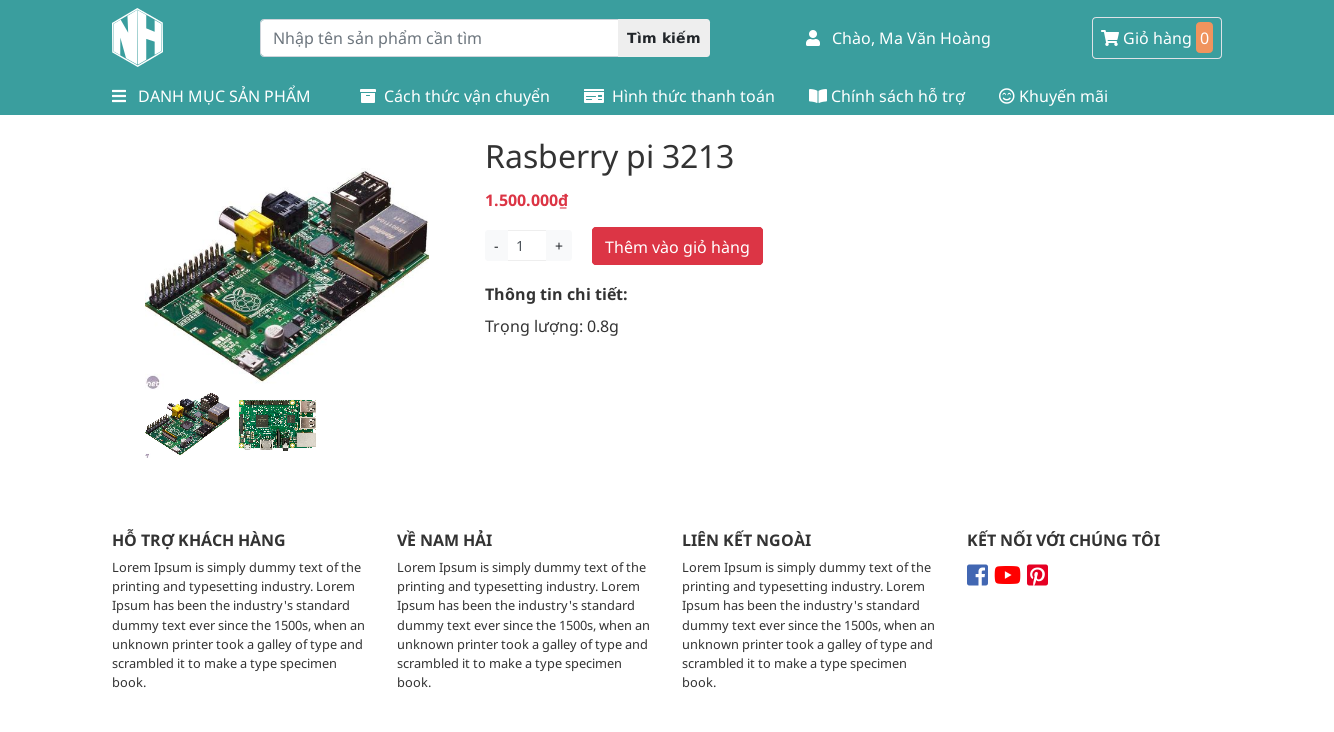
\includegraphics[scale=0.27]{fig/r_product_details.png}
		      \caption{Thiết kế trang chi tiết sản phẩm}
	      \end{figure}
	      \newpage
	\item Giỏ hàng
	      \begin{figure}[h!]
		      \centering
		      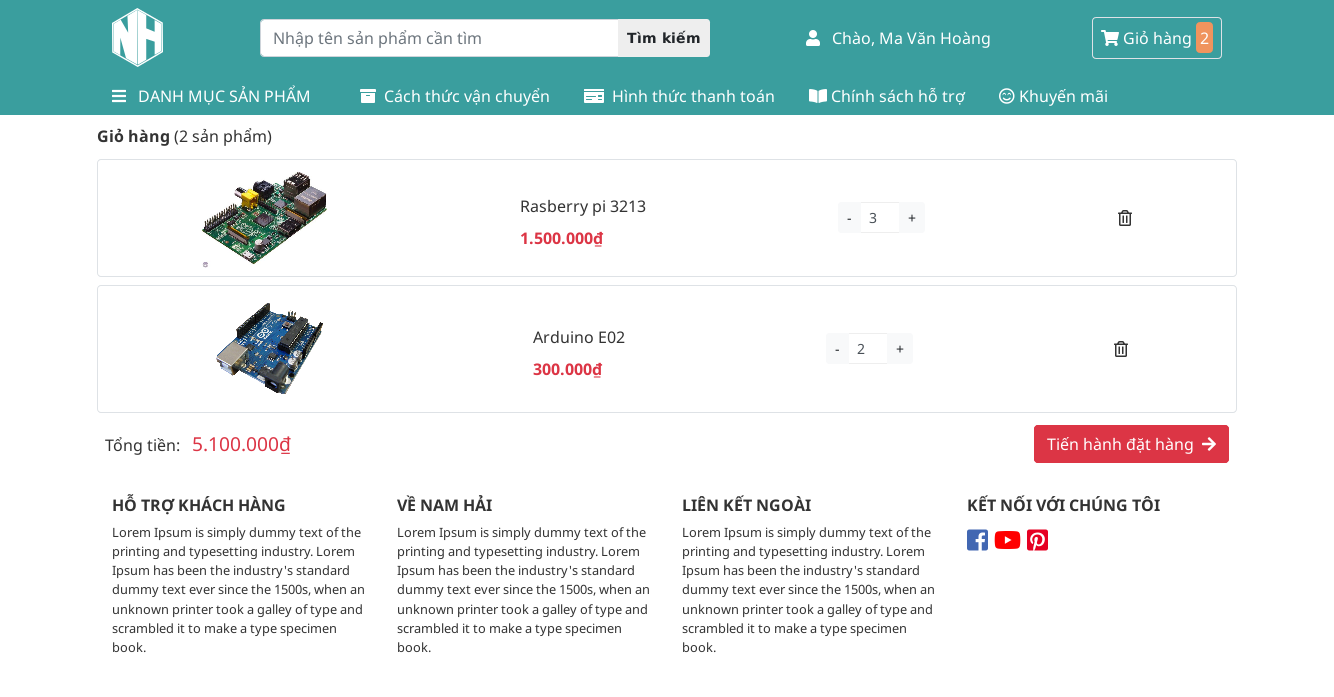
\includegraphics[width=\linewidth]{fig/r_cart.png}
		      \caption{Thiết kế trang giỏ hàng}
	      \end{figure}
	\item Tạo hóa đơn
	      \begin{figure}[h!]
		      \centering
		      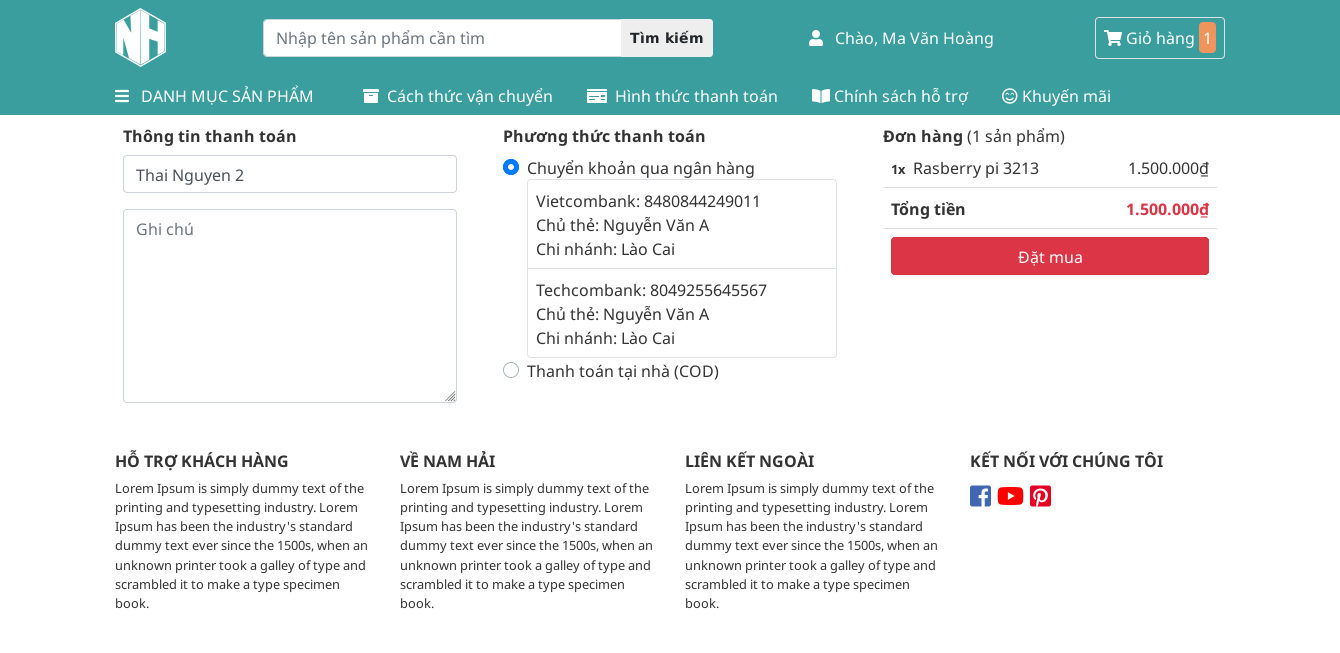
\includegraphics[width=\linewidth]{fig/r_make_order.png}
		      \caption{Thiết kế trang tạo hóa đơn}
	      \end{figure}
	      \newpage
	\item Lịch sử giao dịch
	      \begin{figure}[h!]
		      \centering
		      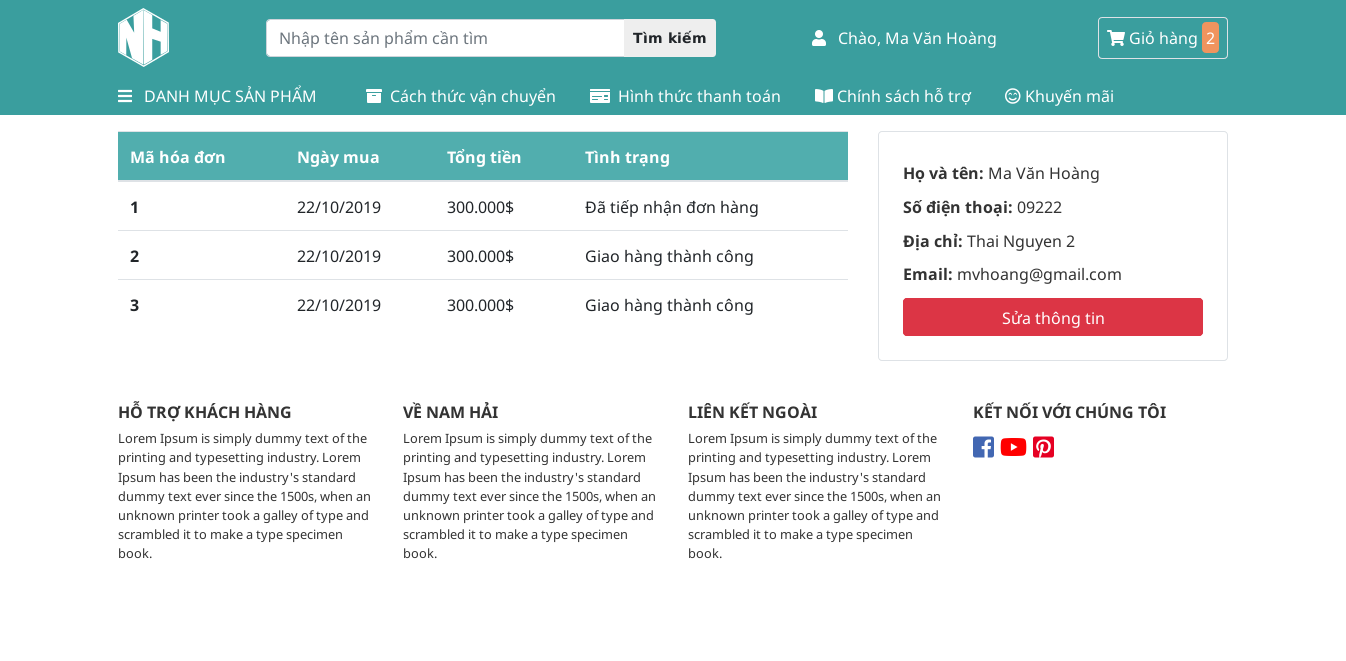
\includegraphics[width=\linewidth]{fig/r_user1.png}
		      \caption{Thiết kế trang lịch sử giao dịch}
	      \end{figure}
	\item Cập nhật thông tin cá nhân
	      \begin{figure}[h!]
		      \centering
		      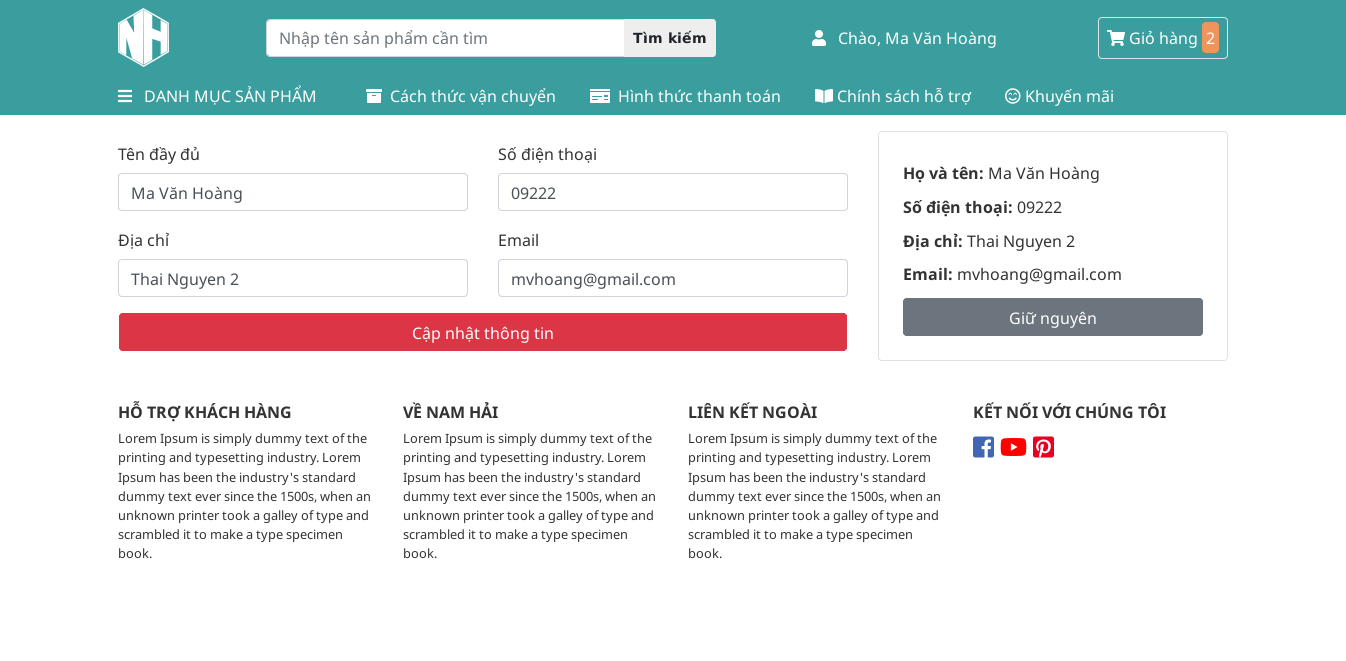
\includegraphics[width=\linewidth]{fig/r_user2.png}
		      \caption{Thiết kế trang cập nhật thông tin cá nhân}
	      \end{figure}
	      \newpage
	\item Trang thống kê
	      \begin{figure}[h!]
		      \centering
		      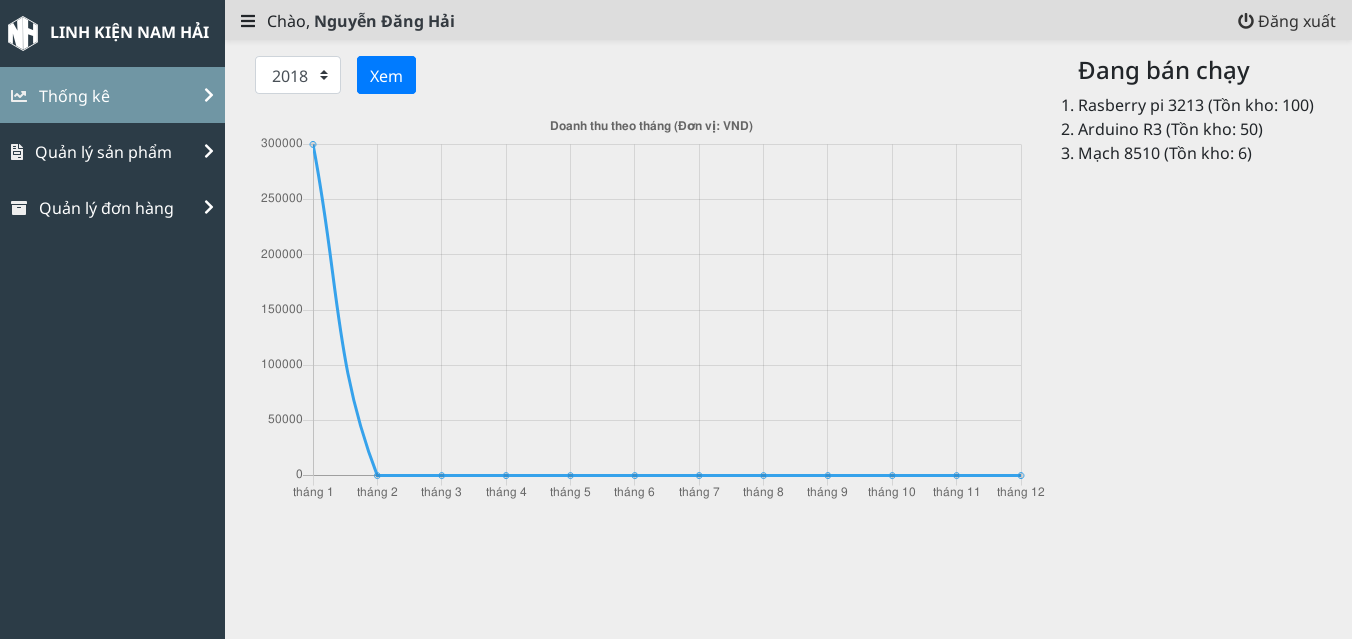
\includegraphics[width=\linewidth]{fig/r_manage_statistics.png}
		      \caption{Thiết kế trang thống kê}
	      \end{figure}
	\item Trang quản lý sản phẩm
	      \begin{figure}[h!]
		      \centering
		      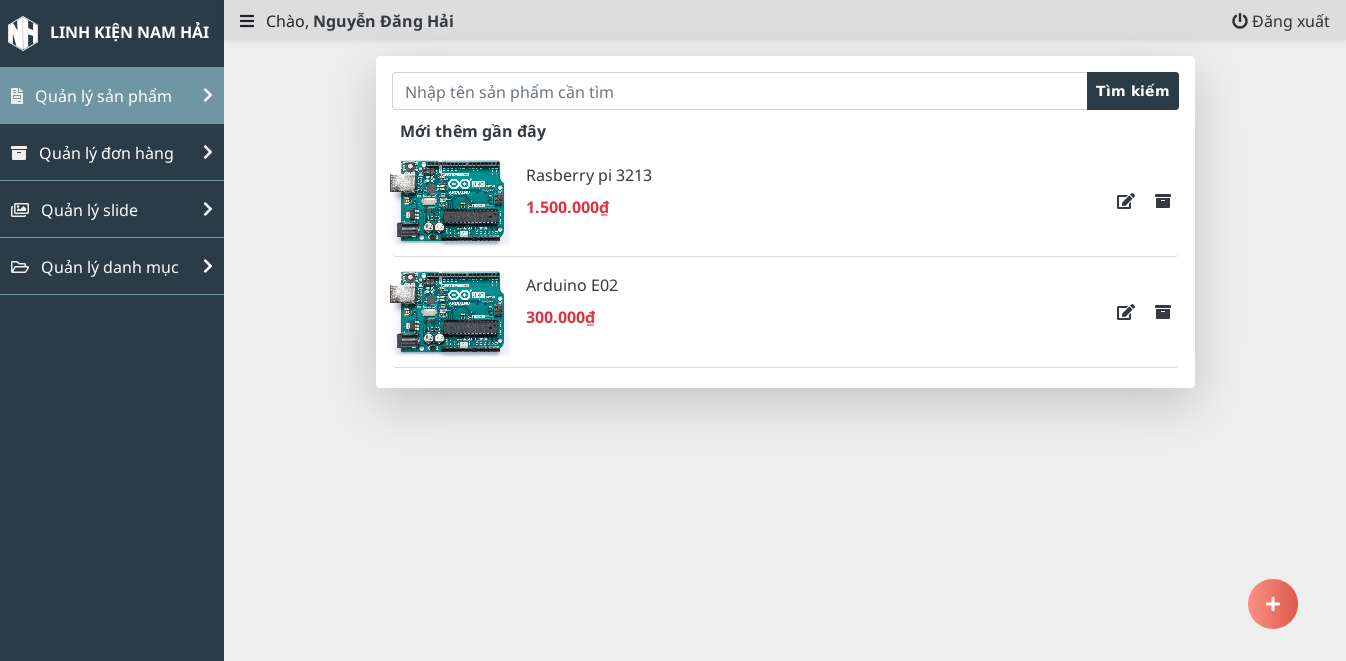
\includegraphics[width=\linewidth]{fig/r_manage_product.png}
		      \caption{Thiết kế trang quản lý sản phẩm}
	      \end{figure}
          \newpage
	\item Trang thêm sản phẩm
	      \begin{figure}[h!]
		      \centering
		      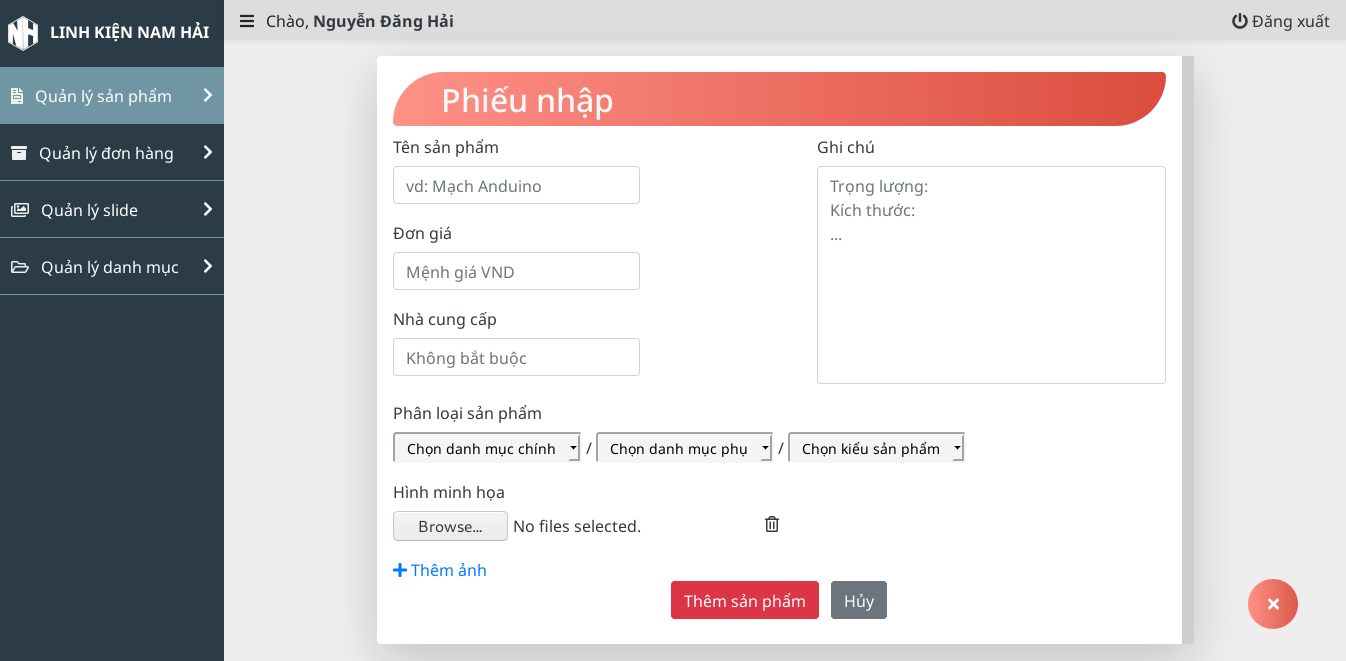
\includegraphics[width=\linewidth]{fig/r_manage_product_add_product.png}
		      \caption{Thiết kế trang quản thêm sản phẩm}
	      \end{figure}
	\item trang cập nhật thông tin sản phẩm
	      \begin{figure}[h!]
		      \centering
		      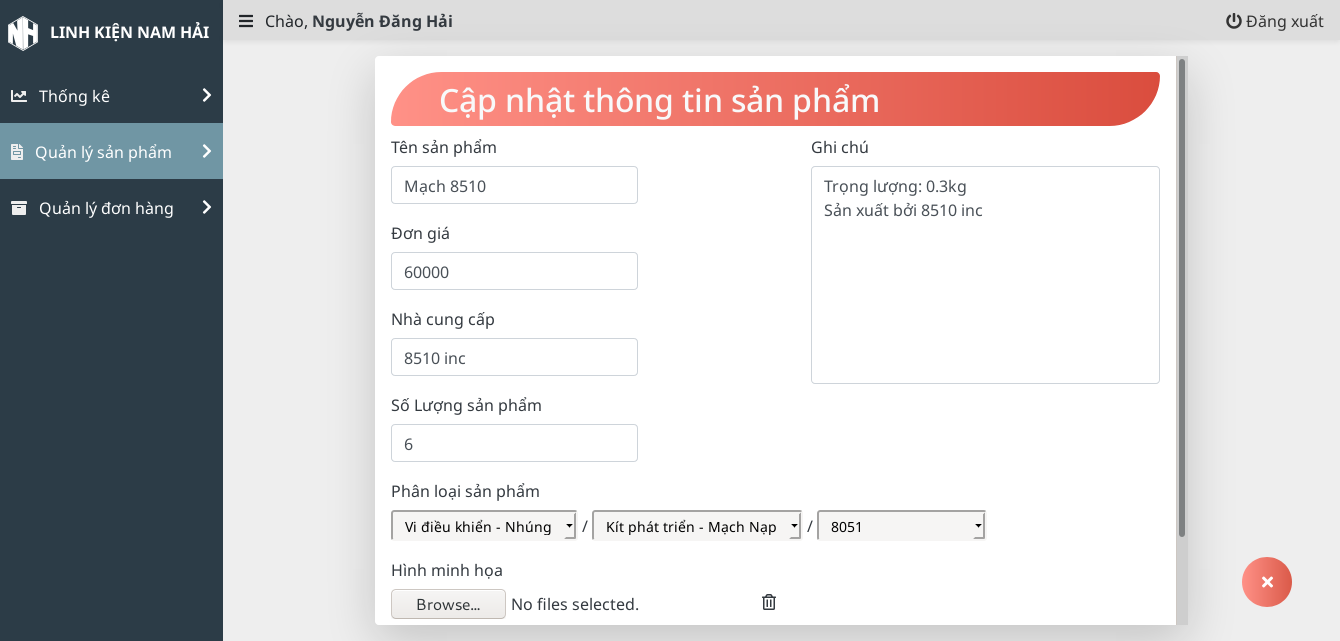
\includegraphics[width=\linewidth]{fig/r_manage_product_update_product.png}
		      \caption{thiết kế trang cập nhật thông tin sản phẩm}
	      \end{figure}
          \newpage
	\item trang quản lý hóa đơn
	      \begin{figure}[h!]
		      \centering
		      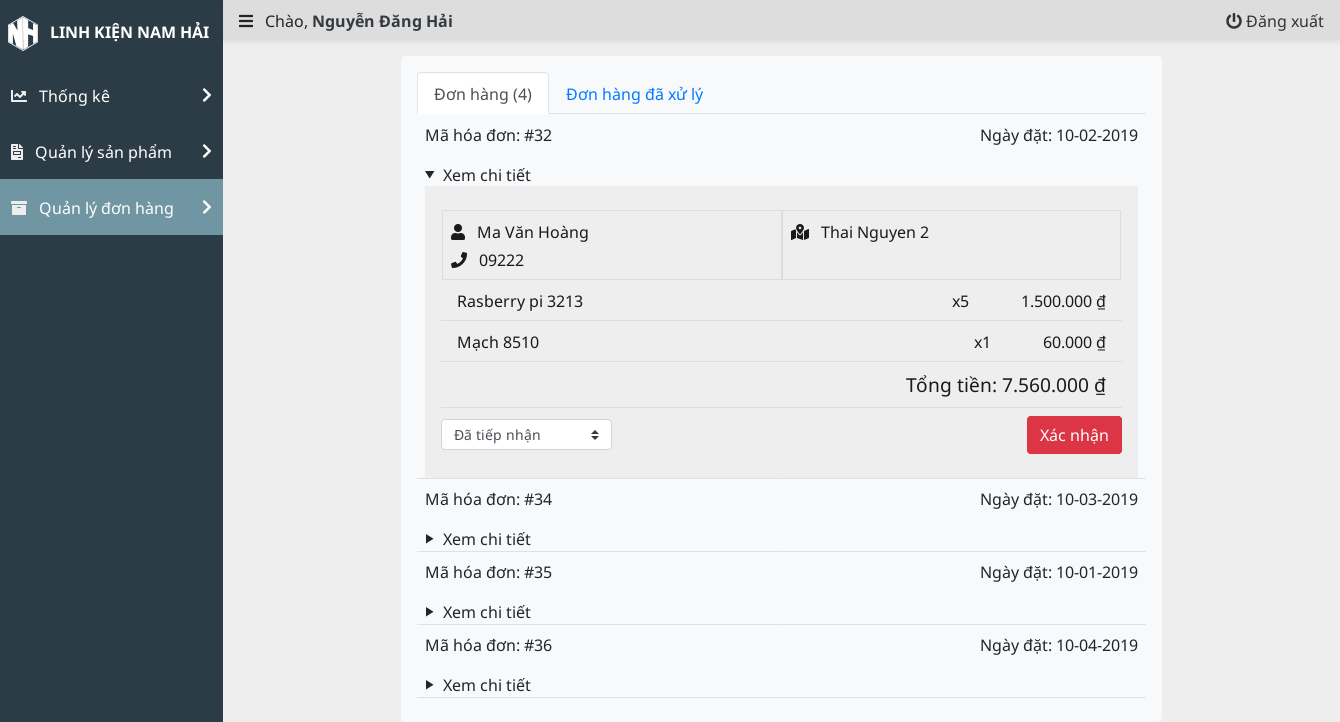
\includegraphics[width=\linewidth]{fig/r_order.png}
		      \caption{thiết kế trang quản lý hóa đơn}
	      \end{figure}
          \newpage
\end{enumerate}

\addcontentsline{toc}{chapter}{Kết luận}
\noindent\textbf{Kết luận}

\textbf{Kết quả đạt được}

Thông qua quá trình thực hiện đề tài em đã hiểu hơn về các ngôn ngữ lập
trình web như HTML, CSS, PHP và một số kỹ thuật lập trình web như Ajax và
MVC.

Hiện tại website trò chuyện trực tuyến của em đã có thể thực hiện một số chức năng chính như:
\begin{itemize}
    \vspace{-1em}
    \itemsep0em
    \item đăng ký, đăng nhập, cập nhật thông tin cá nhân.
    \item tìm kiếm sản phẩm.
    \item phân quyền truy cập.
    \item xem thống kê doanh thu và xem sản phẩm được mua nhiều.
    \item quản lý sản phẩm, quản lý hóa đơn.
    \vspace{-1em}
\end{itemize}

\textbf{Hướng phát triển}

Trong tương lai, em sẽ tích hợp và phát triển thêm một số tính năng như:

\begin{itemize}
    \vspace{-1em}
    \itemsep0em
    \item quên mật khẩu
    \item gửi email chứa thông tin hóa đơn tới địa chỉ email được khách hàng cung cấp
    \item cải thiện cấu trúc của code để dễ dàng nâng cấp và sửa chữa hơn
    \vspace{-1em}
\end{itemize}

\clearpage
\phantomsection
\renewcommand{\bibtex}{Tài liệu tham khảo}
\bibliographystyle{ieeetr}
\bibliography{bibtex/biblio}
\clearpage
\addcontentsline{toc}{chapter}{Nhận xét của giáo viên}
\begin{center}
    \textbf{Nhận xét của giáo viên}
\end{center}


\end{document}
